\documentclass[11pt,a4paper]{book}
\usepackage[utf8]{inputenc}
\usepackage[spanish]{babel}
\renewcommand{\spanishlisttablename}{Índice de tablas}
\renewcommand\spanishtablename{Tabla}
\usepackage{amsmath}
\usepackage{amsfonts}
\usepackage{graphicx}
\usepackage{amssymb}
\usepackage[left=2cm,right=2cm,top=2cm,bottom=2cm]{geometry}
\usepackage{cite}
\usepackage{babelbib}
\usepackage{float}
\author{Víctor de Tejada Molera}

\begin{document}

\tableofcontents
\listoffigures
\listoftables

\chapter{Estado del arte}
    En este capítulo se pretende realizar un análisis del estado del arte referente a los experimentos psicoacústicos; concretamente aquellos que se centran principalmente en la evaluación de diferencias perceptuales en entornos cerrados como auditorios, cines, salas de conferencias, etc.
    
    Para la búsqueda de esta información, se recurre a bases de datos científicas como el sistema \textit{Ingenio UPM} y buscadores de artículos científicos como \textit{Google Scholar}. Con ellos, se han introducido términos de búsqueda como ``\textit{Psychoacoustics}'', ``\textit{Subjective test acoustics}'' o ``\textit{Auditorium subjective test}''. Los resultados arrojados por dichas plataformas, se revisan y se lee el resumen o \textit{abstract} de los que se consideran que pueden ser útiles para el proyecto. Si el resumen confirma que la temática concuerda con la del estudio, se procede a la lectura del resto del artículo y se extraen los elementos que se consideran más importantes. Estos son principalmente: el tipo de análisis estadístico que se ha utilizado, el número de personas que han realizado el test, el tipo de test (tipo de preguntas, formato, duración de los audios utilizados, etc.), entre otros.
    
    Por otro lado, se ha realizado, paralelamente, una búsqueda de fuentes bibliográficas especializados en temas como de detección de señales, análisis estadístico de datos y, más específicamente, sobre modelos Thurstonianos. Para ello, se realizan nuevas consultas a los medios ya presentados a personas con experiencia contrastasda en la realización y el estudio de experimentos psicoacústicos.\newline
    
    Utilizando estos medios, se han consultado alrededor de 30 documentos entre libros de referencia, normativas internacionales, artículos en revistas y congresos, trabajos de fin de grado, etc. En ellos, como se menciona en \cite{Tejada2020}, las características de los test subjetivos aplicados son muy diferentes entre sí e incluyen una gran variedad en cuanto al número de participantes o procedimientos se refiere.
    
    \section{Análisis de la documentación consultada}
    
    Al observar los distintos documentos, se ha observado una gran inconsistencia en las características de los diferentes estudios que se han analizado. En este apartado se analizan las características de los proyectos y normativas según varios de sus aspectos más representativos. 
    
    
    
	    \subsection{Número de participantes}
    		Si se analizan las características de las personas que participan en los test perceptuales, se observa una gran variedad tanto en el número como en su experiencia. 
    		
    		Por un lado, se tienen estudios que utilizan un número muy pequeño de personas, diez o menos, como es el caso de \cite{2019MNowak}. Por otro lado, algunos casos presentan números mucho mayores llegando a utilizar casi cien personas, como ocurre en \cite{1954JEgan}. También se observa que el número de participantes varía en función del aspecto subjetivo que pretenda analizarse \cite{Tejada2020}; de esta forma, los estudios que estudian la molestia acústica son los que utilizan un mayor número de participantes (en torno a los 30-40 según \cite{Tejada2020}), mientras que el resto utilizan unas 20 personas aproximadamente, que se corresponde con las recomendaciones de las normativas \cite{UIT1116, UIT1284, UIT1534}.

            Otro aspecto importante muy relacionado con el número de participantes consiste en la utilización de participantes con o sin experiencia en este tipo de experimentos psicoacústicos. Normativas como \cite{UIT1116, UIT1284, UIT1534} recomiendan la utilización de participantes con experiencia cuando los aspectos a analizar son bastante técnicos o requieren de personas con oídos especializados en la detección de ciertos eventos. No obstante, aceptan la presencia de participantes sin experiencia si se aumenta el número total de personas que participan en el experimento o si se les aplica algún tipo de entrenamiento previo, incluso se recomienda realizarlo para participantes con experiencia.

            A pesar de estas recomendaciones, la realidad es bastante diversas en la que se encuentran estudios como \cite{1995GASoulodre,1999JBradley, 2005IWitew, 2010FMartellotta, 2010MVigeant, 1997SCarlile, 2011VEmiya, 2016BPostma, 2019ZShao, 2019VRajala, 2019MShiell, 2019JGroose, Braun2004, delaPrida2019, delaPrida2021} en los que sí se aplican entrenamientos previos, mientras que en otros estudios como \cite{Brockhoff2009,2019LKritly,2019DMorikawa, 2019DJSchlit} no se realizan. También se han encontrado varios estudios en los que no se reflejaba si se habían realizado estos entrenamientos o no \cite{2002PZahorik, 2016SKlockgether, 2019GPulvirenti,2019MNowak, 2019MYamada, 2019JLee, Christensen2009}.
    
	    \subsection{Interacción por parte del participante}
    		A nivel de interacción por parte de la persona participante, existe división de opiniones sobre la posibilidad del usuario de poder controlar la reproducción de los estímulos \cite{1995GASoulodre, 2010FMartellotta, 2010MVigeant, 2011VEmiya,2019DMorikawa} frente a \cite{1999JBradley, 2002PZahorik, 2005IWitew, 2016SKlockgether, 2019VRajala, 2019VHongisto} No obstante, normas como \cite{UIT1116,UIT1534, UIT1284,EBU3286, UIT1285, UIT1286} recomiendan que los participantes tengan, siempre que sea posible, la capacidad de interactuar con los estímulos de forma directa y repetir su reproducción si así lo desean.

	    \subsection{Aspectos subjetivos a analizar}
		    Los aspectos subjetivos que se pueden analizar mediante test perceptuales son muy variados. Por un lado algunos experimentos como en \cite{1995GASoulodre, 2016SKlockgether,  2016BPostma, 2002PZahorik} se centran en estudiar las características relacionadas con la reverberación de las salas (persistencia del sonido, diferencias entre sonidos anecoicos y reverberantes, etc.). Otros estudios se centran en el estudio d ela inteligibilidad de diferentes señales acústicas \cite{ 1999JBradley, 2010FMartellotta,  2010MVigeant}, mientras otras se centran en temas de localización de sonora \cite{1997SCarlile, 2019MShiell, 2019MYamada, 2019DMorikawa}. También se encuentran aquellos experimentos en los que se pretende estudiar características como las diferencias entre señales, la sonoridad o diferencias de nivel \cite{2019GPulvirenti, 2016SKlockgether, 2019MNowak, 2011VEmiya, 2019LKritly, 2005IWitew,  2019DJSchlit}. Por último, una de las áreas que está teniendo más importancia en los últimos años se corresponden con el estudio de la molestia acústica \cite{2019VHongisto, 2019JLee, 2019VRajala}.
		    
            Algunos documentos com \cite{Tejada2020} tratan de ordenar estos documentos en diferentes categorías y facilitar el análisis de grandes cantidades de documentos y extraer sus elementos comunes.

	    \subsection{Tipos de test}
    		Por otro lado, se ha observado una gran variedad de formatos para hacer los test. Los más habituales se presentan a continuación.
    
    		\begin{itemize}
        		\item \textbf{Test de diferencias}: En este tipo de test al oyente se le presentan 2 o más audios y tiene que determinar si son iguales o no. Tiene la ventaja de que son sencillos de implementar y de analizar. En algunos sitios, se le llama ``Duo'' o ``binomial'' por lo que es importante revisarlos a conciencia para no confundirlos con los ``Duo-Trio'' o un ``ABX''. Algunos de los artículos en los que han aplicado este tipo de test son \cite{1995GASoulodre, 1999JBradley,2002PZahorik, 2005IWitew, 2010MVigeant, 2019LKritly}.
        		\item \textbf{Test Duo-Trio}: Para este formato, se presentan tres audios. Uno de ellos es igual a  uno de los otros dos que se denomina ``Referencia''. El objetivo del oyente es determinar cuál de los audios que se le presenta es igual a dicha referencia. Algunos de los proyectos que han utilizado este tipo de test son \cite{delaPrida2019, delaPrida2021}.
        		\item \textbf{Test de escalas numéricas}: El objetivo de este test es que el oyente cuantifique alguna determinada característica de las señales de audio mediante una escala numérica. Algunas variantes permiten que se realice la cuantificación de varios elementos en paralelo o que se pida que se ordenen varios audios simultáneamente en función de la característica que se pretenda evaluar (Test de MUSHRA \cite{UIT1534}). Este tipo de test son muy útiles y aparecen como recomendación por parte de normativas internacionales \cite{UIT1116, UIT1284, UIT1534}.También aparecen en algunos documentos como \cite{2011VEmiya,2016BPostma, 2019ZShao,2019GPulvirenti,2019VRajala, 2019JLee, 2019DMorikawa}. 
        		\item \textbf{ABX}: En este tipo de test se presentan tres señales. El oyente tiene que determinar cuál de las dos primeras que se le presentan es igual a la que es presentada en último lugar. El experimento se repite varias veces modificando la última señal para que no sea siempre el mismo audio. Algunos ejemplos donde se aplican este tipo de test se encuentran en \cite{delaPrida2021, Braun2004}.
    		\end{itemize}
    		Existen otros tipos de test como los triangulares o los A/NotA que se reflejan y explican en \cite{delaPrida2021, Brockhoff2009}. No obstante, no se han encontrado experimentos en los que se aplique dicha metodología, a parte de ese artículo, por lo que no se han considerado para las siguientes partes del proyecto.
    
    		Cada uno de los tipos de test mencionandos arriba tienen sus propias particularidades, sus ventajas y sus inconvenientes tanto para su realización como para el análisis de sus resultados.
    
	

        \subsection{Duración del experimento}
    		En cuanto a la duración de los estímulos, se han observado que los valores suelen rondar de 1 a 5 segundos \cite{2010FMartellotta, 2016SKlockgether, 2011VEmiya, 2019LKritly, 2019GPulvirenti, 2002PZahorik, 2019MShiell, 2019JGroose, 2019MNowak, 2019MYamada, 2019DMorikawa, 2019DJSchlit}. No obstante, también se han encontrado estudios donde la duración se encuentra entre los 8-10 segundos \cite{2010FMartellotta, 2019JLee, 2010MVigeant}, obteniéndose casos con un máximo de 15 segundos como en \cite{1995GASoulodre, 2005IWitew}. Esto concuerda con las recomendaciones de \cite{UIT1116,UIT1534, UIT1284,EBU3286, UIT1285, UIT1286} al respecto donde se indica que la duración de dichos estímulos debe ser lo suficientemente reducida para evitar que los participantes se acostumbren a las señales \cite{GelfandStanley}. Unido a esto, la duración total de la sesión, a pesar de ser el apartado del que menos información se aporta, se recomienda que no exceda de los 30 minutos , siendo necesaria la inclusión de descansos de la misma duración, si se tiene que alargar \cite{UIT1116, UIT1284, UIT1534, ZwickerFactsModels, GelfandStanley, BlauertSpatialHearing}. Esto ocurre en casos como \cite{2019LKritly} donde se tiene una duración de casi 90 minutos.
    
	    \subsection{Análisis de los datos}
    		En cuanto al análisis de los datos, históricamente se han utilizado procedimientos como los análisis de la varianza (ANOVA) \cite{2011VEmiya, 2016BPostma, 2019LKritly, 2019GPulvirenti, 2019MShiell, 2019VHongisto}, o normas como \cite{ISO10399}. No obstante, en estudios más recientes como \cite{delaPrida2019, delaPrida2021} aparecen los modelos thursthonianos como una alternativa sencilla de aplicar y con cualidades que pueden resultar útiles para ciertos tipos de estudio.\newline
    
    A la vista de todo lo expuesto, queda patente la gran variedad de sistemas que se siguen en la actualidad para realizar los test perceptuales. Por ello, para nuestro test es necesario identificar sus particularidades para poder determinar las características que mejor se ajusten al mismo. 
    
    \section{Conceptos teóricos para el análisis estadístico}    
        \subsection{UNE-EN ISO 10399}
            La norma UNE-EN ISO 10399: ``Análisis sensorial. Metodología. Ensayo Duo-Trio.''\cite{ISO10399} es un documento que permite analizar la probabilidad de que eventos perceptuales sean percibidos como iguales o diferentes según el número de respuestas definidas como correctas y/o erróneas al realizar experimentos basados en test duo-trio.
        
            Para ello, en primer lugar se definen diferentes términos que aparecen de forma constante a lo largo de la norma. Para nuestro caso particular, los términos más relevantes son:
        
            \begin{itemize}
                \item alpha-risk o $\alpha$-risk: es la probabilidad para poder afirmar que existe una diferencia perceptual cuando en realidad no existe.
                \item beta-risk o $\beta$-risk: es la probabilidad para poder afirmar que no existe una diferencia perceptual cuando en realidad sí existe.
                \item diferencia perceptual: situación en la que dos o maś muestras pueden ser distinguidas por sus propiedades sensitivas (a través del oído, tacto, gusto, vista, etc.)
                \item similaridad perceptual: situación en la que las diferencias entre muestras son tan pequeñas que no pueden distinguirse entre sí de forma sensitiva.
            \end{itemize}
            Para el cálculo de las probabilidades $\alpha$-risk y $\beta$-risk, la norma proporciona sendas tablas que se encuentran en el Anexo A de dicha norma (las tablas A.1 y A.2 respectivamente). También se proporciona la ecuación \ref{eq:alpha} donde se puede calcular el mínimo de respuestas ``correctas'' para que se obtenga un determinado valor de $\alpha$-risk.
            
            \begin{equation}
                x=(n/2)+z*\sqrt{n/4}
                \label{eq:alpha}
            \end{equation}
            
            Donde:
            \begin{itemize}
                \item x: número de respuestas correctas mínimas necesarias para que se obtenga un determinado $\alpha$-risk.
                \item n: número de respuestas totales.
                \item z: variable que toma un valor en función de $\alpha$-risk:
                \begin{itemize}
                    \item 0.84 para $\alpha=0.20$.
                    \item 1.28 para $\alpha=0.10$.
                    \item 1.64 para $\alpha=0.05$.
                    \item 2.33 para $\alpha=0.01$.
                    \item 3.09 para $\alpha=0.001$.
                    
                \end{itemize}
            \end{itemize}
            
            Un ejemplo de aplicación para conocer el coeficiente $\alpha$-risk sería el siguiente: Suponemos que tenemos un caso de estudio entre dos señales acústicas.  Se ha realizado un test perceptual y se han obtenido 100 respuestas, 87 de las cuales se ha obtenido que las dos señales son diferentes.
            
            En primer lugar, se acude a la tabla del Anexo A.1 para comprobar si están los datos para ese número de respuestas. En este caso, se comprueba que, desgraciadamente, la tabla sólo arroja datos hata las 88 respuestas, por lo que se procede a resolver la ecuación \ref{eq:alpha}. Sustituyendo las variables por los datos que se tienen, se obtienen 5 valores diferentes de x para cada uno de los posibles valores de $\alpha$:
            \begin{itemize}
                \item $x=55$ para $\alpha=0.20$.
                \item $x=57$ para $\alpha=0.10$.
                \item $x=59$ para $\alpha=0.05$.
                \item $x=62$ para $\alpha=0.01$.
                \item $x=66$ para $\alpha=0.001$.
            \end{itemize}
            Es importante remarcar que los resultados siempre se redondean hacia arriba, puesto que es imposible tener fracciones de respuestas.
            
            Una vez obtenidos los valores, el valor de $\alpha$ se corresponde con el del caso más cercano que sea inferior a nuestro número de respuestas diferentes. En nuestro caso, $\alpha=0.001$ ya que 66 es el número más cercano a 87 (y además se cumple de que es menor).
            
            Como ya se explicó anteriormente, el coeficiente $\alpha$-risk muestra la probabilidad de que dos eventos sean diferentes cuando, en realidad, son iguales. Por este motivo, cuanto más pequeño es el valor del coeficiente, más estadísticamente representativa es la diferencia perceptual. Por este motivo, en estudios como el nuestro, se busca obtener valores pequeños.
            
            Puede ocurrir que se obtengan situaciones donde el número de respuestas en las que se han indicado que son diferentes sea menor que para el caso de $\alpha=0.20$ (en el ejemplo anterior, si se hubiera obtenido menos de 55 respuestas marcadas como diferentes). Si este fuera el caso, no se podría concluir que estadísticamente la percepción de dichos estímulos es diferente. En todo caso, habría que concluir que las posibles diferencias son debidas al azar. 
            
        \subsection{Modelos Thursthonianos}
            Los modelos Thursthonianos\cite{PsychophysicsB, SignalB, delaPrida2019} son modelos estadísticos en los que se utilizan variables de distribuciones normales y que se utilizan en gran medida en estudios de discriminación sensorial. 
            
            En el caso concreto de la psicoacústica, se utilizan generalmente para obtener un valor ``$d'$'' que da información ordenada y cuantitativa sobre una determinada percepción subjetiva. Además de este valor, se calcula a su vez la desviación estandar ``$\sigma$''. Con estos dos valores, se puede aproximar las respuestas de un test subjetivo como una sucesión de distribuciones gaussianas en las que en función del valor ``$d'$''y ``$\sigma$'' están más o menos superpuestas. Esta superposición da información sobre la probabilidad de que ambos estímulos puedan ser distinguibles o no entre sí y cuánto. Esto se observa más fácilmente en la figura \ref{fig:modelost} obtenida en \cite{PsychophysicsB}.
            
            \begin{figure}[H]
                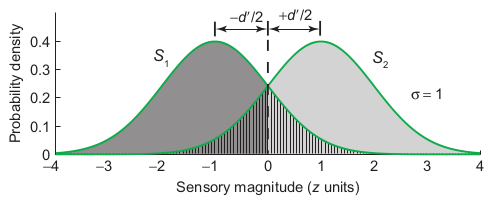
\includegraphics[scale=0.7]{../imagenes/modelosthurst.png}
			    \centering
			    \caption{Ejemplo de cálculo de $d'$ utilizando modelos thursthonianos. Fte: \cite{PsychophysicsB} }
			    \label{fig:modelost}
            \end{figure}
            
            Utilizando la figura \ref{fig:modelost} como ejemplo, se puede suponer que S1 y S2 son las distribuciones obtenidas de las respuestas de un test en las que S1 son las respuestas en las que dos estímulos han sido identificados como iguales, mientras que S2 se corresponde con las respuestas cuando los dos estímulos se identifican como diferentes. Cuanto más se solapen ambas distribuciones, más difícil será para los participantes distinguirlas. Gráficamente resulta fácil comprobar que las variables que determinan este solapamiento es principalemente $d'$, sin dejar de lado la importancia que tiene la desviación estándar $\sigma$.
            
            Además de lo ya expuesto, este tipo de análisis es especialmente interesante porque nos permite ordenar los valores obtenidos para $d'$ de forma que las diferencias entre ellos nos da información cuantitativa sobre cómo de diferentes o de similares son cada una de las distribuciones. Con la facilidad añadida que tiene este sistema para representar gráficamente mediante las técnicas habituales como diagramas de barras, entre otros. También tiene la ventaja de que el valor del coeficiente $d'$ es independiente del tipo de test que se realice, incluso es posible compararlos entre sí \cite{delaPrida2021}.
    
    \chapter{Toma de datos}
	Para la realización de este proyecto, es necesaria la obtención de un gran número de respuestas al impulso en diferentes posiciones de una sala. En este capítulo, se repasan y analizan los criterios seguidos para la toma de los datos que posteriormente son procesados y utilizados en el test subjetivo de audio. Del mismo modo, se comenta el espacio escogido para la toma de los datos y el equipo utilizado.

	\section{Localización}

		\subsection{Descripción del espacio}

 			En nuestro caso particular, se ha optado por el auditorio de la ETSIST ubicada en el Campus Sur de la UPM. Este salón de actos está diseñado como sala de conferencias y como espacio para actuaciones de música coral. 
 
 			El espacio tiene unas dimensiones de 25 metros de largo, por 13.64 metros de ancho. El auditorio tiene una altura aproximada de unos 5 metros. En la figura \ref{fig:auditorio} puede observarse la vista en planta de la sala junto a sus diferentes zonas.
 			
 			\begin{figure}
				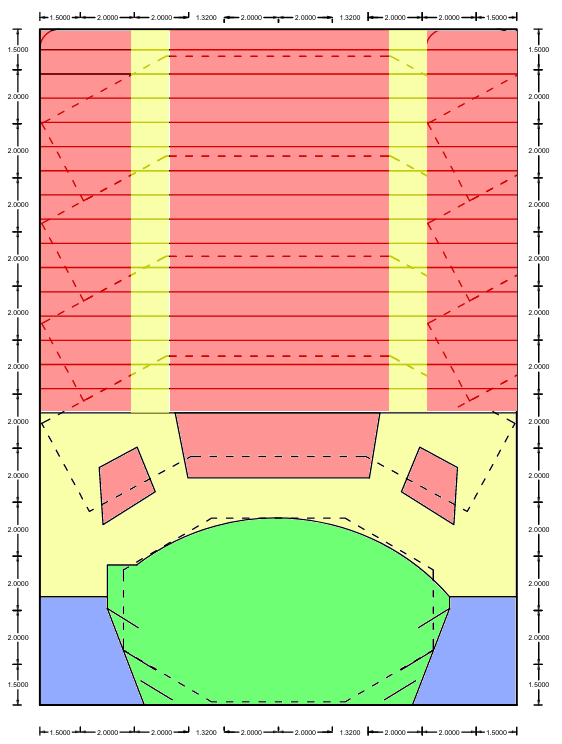
\includegraphics[scale=0.6]{../imagenes/auditorioColor.png}
				\centering
				\caption{Vista en planta del auditorio de la ETSIST. La zona verde se corresponde con el escenario. La zona roja con el patio de butacas. La zona amarilla con los pasillos y zonas de paso. La zona azul son las bambalinas laterales. Las lineas discontínuas marcan la superficie de la concha acústica y los paneles de madera del techo.}
				\label{fig:auditorio}
			\end{figure}
 
 			El escenario se encuentra ligéramente levantado sobre el suelo del salón de actos mediante una estructura de madera. A los lados del escenario se encuentran unos paneles giratorios, también de madera, que dan acceso a dos bambalinas laterales. La parte trasera del escenario cuenta con un gran panel de madera situado en el centro de la pared. El techo del escenario cuenta con una concha acústica de madera y ocupa practicamente toda su superficie. El resto del techo se compone de paneles de madera ligeramente superpuestos y con ligera inclinación para evitar superficies paralelas.
 
 			Las paredes del auditorio se encuentran recubiertas en su mayoría por paneles de madera, excepto por una ligera zona acristalada hacia la zona superior. Las puertas situadas en los laterales son metálicas. 
 
 			La pared posterior, así como el resto de las paredes están compuestas principalmente de \textit{hydropanel} y láminas de madera. En la parte trasera también se encuentra una puerta metálica y una ventana acristalada que comunican con la sala de control.
 
 			El suelo de la zona más cercana al escenario está compuesto por láminas de madera, mientras que en la zona de butacas, se compone de linóleo.
 			
 			Finalmente, el patio de butacas está constituido por 485 asientos individuales tapizados de material textil y rellenos de material esponjoso que no se ha podido consultar.
 
 			Estos materiales pueden observarse en la figura \ref{fig:materiales}.
 
 			\begin{figure}
 				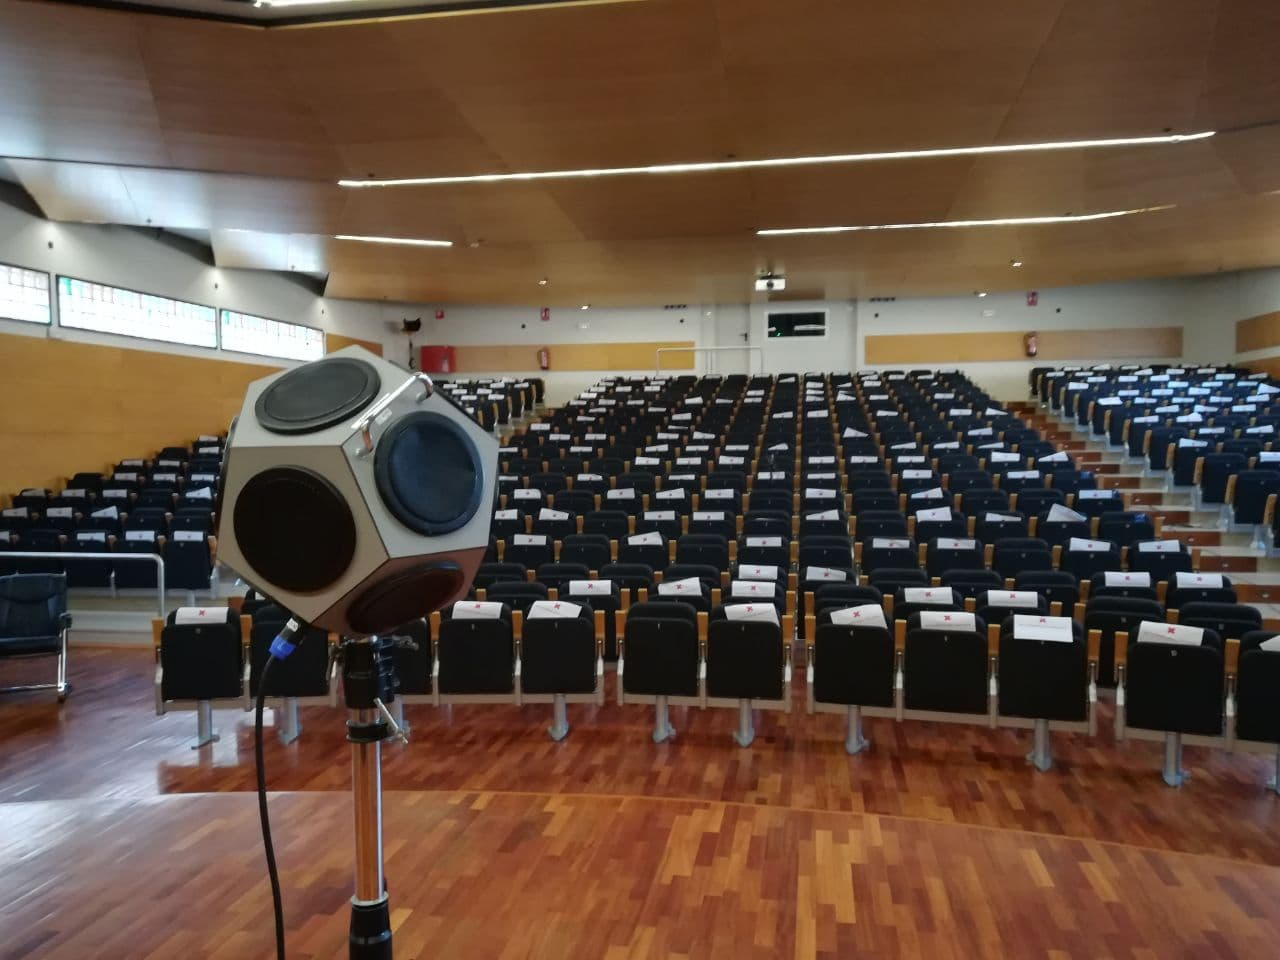
\includegraphics[scale=.25]{../imagenes/fuente.jpg}%
 				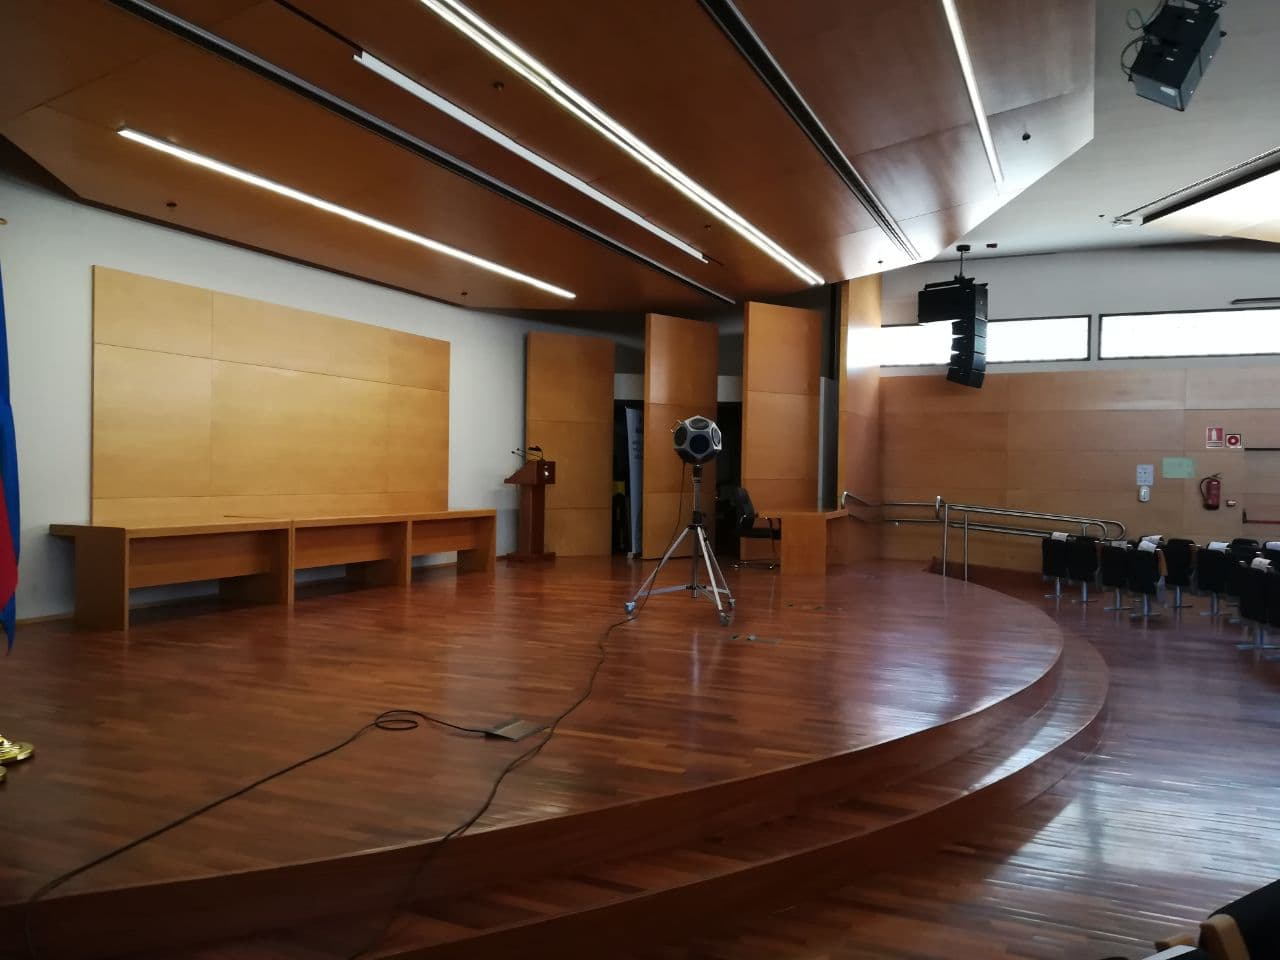
\includegraphics[scale=.25]{../imagenes/fuente2.jpg} 
 				\centering
 				\caption{El auditorio de la ETSIST. Izquierda: patio de butacas visto desde el escenario. Derecha: escenario}
 				\label{fig:materiales}

 			\end{figure}
 


		\subsection{Distribución de las butacas}
			Este espacio está compuesto de dos zonas de butacas distintas:

 			Por un lado, dieciseis filas de butacas paralelas en escalera de veintiocho butacas cada una. Estas butacas se encuentran numeradas desde el centro hacia los extremos; los números pares se encuentran hacia la derecha (mirando desde el escenario ver figura \ref{fig:materiales}) y los números impares se encuentran hacia la zona de la izquierda.
 
 			Por otro lado, existen otras dos filas de butacas situadas por delante del primer grupo. Estas tres filas se encuentran divididas, a su vez, en tres grupos: uno centrado y otro en cada lado (izquierda y derecha). La numeración sigue el mismo orden que las filas mostradas anteriormente. La numeración comienza en el centro del area central y los números pares se incrementan hacia la derecha. Esta numeración continúa en las zonas adyacentes como si se trataran de la misma fila. Se produce una situación análoga con las impares en la zona izquierda del auditorio.
 
 			En la figura \ref{fig:auditorio} se puede observar un esquema en planta del auditorio en el que se aprecian tanto las filas convencionales, como las áreas adicionales.
			
			
    \section{Primera toma de datos}
	    \subsection{Numeración y selección de las posiciones de toma de datos}
		    Como se plantea disponer de un gran número de respuestas al impulso, es importante determinar previamente un sistema para numerar inequívocamente las distintas posiciones en las que se van a tomar los datos. Por suerte, tanto las filas como las butacas ya se encuentran numeradas de antemano. Por ello, se decide mantener esta numeración para almacenar y referencias los datos de cada una de las posiciones. De esta forma, se tiene que para la zona de butacas paralelas la numeración es de la forma: ``FxBy''. Siendo ``x'' el número de la fila en la que se encuentra e ``y'' el número de la butaca.

		    Para la zona delantera, la numeración es ligéramente distinta y es de la forma ``AxBy''. Donde, de nuevo, ``x'' e ``y'' representan el número de fila y butaca respectivamente.

		    De esta forma, dos ejemplos pueden ser ``F3B27'' y ``A2B8''; siendo las posiciones de la butaca 27 de la fila 3 de butacas paralelas y la butaca 8 de la fila 3 de la zona delantera, respectivamente.

		    Con esta forma de numeración de butacas, se puede proceder a la selección de las diferentes posiciones en las que se obtienen las respuestas impulsivas de la sala. Para el caso de este proyecto, se ha supuesto que el salón de actos es simétrico en la parte izquierda y derecha. Por este motivo, se han determinado posiciones en la parte par de la sala. Después, se ha distribuido el área seleccionando una butaca y dejando butacas libres antes de seleccionar la siguiente posición para cada fila. Así mismo, para la fila siguiente no se selecciona la butaca que está en frente de la seleccionada, sino la inmediatamente a continuación a su derecha. De esta forma, se consigue un muestreo más uniforme de la sala. En total se tomaron 100 grabaciones en esta primera toma de datos y en la figura \ref{fig:butacasMarcadas} puede observarse un esquema con dicha distribución. 
		
		    \begin{figure}
	            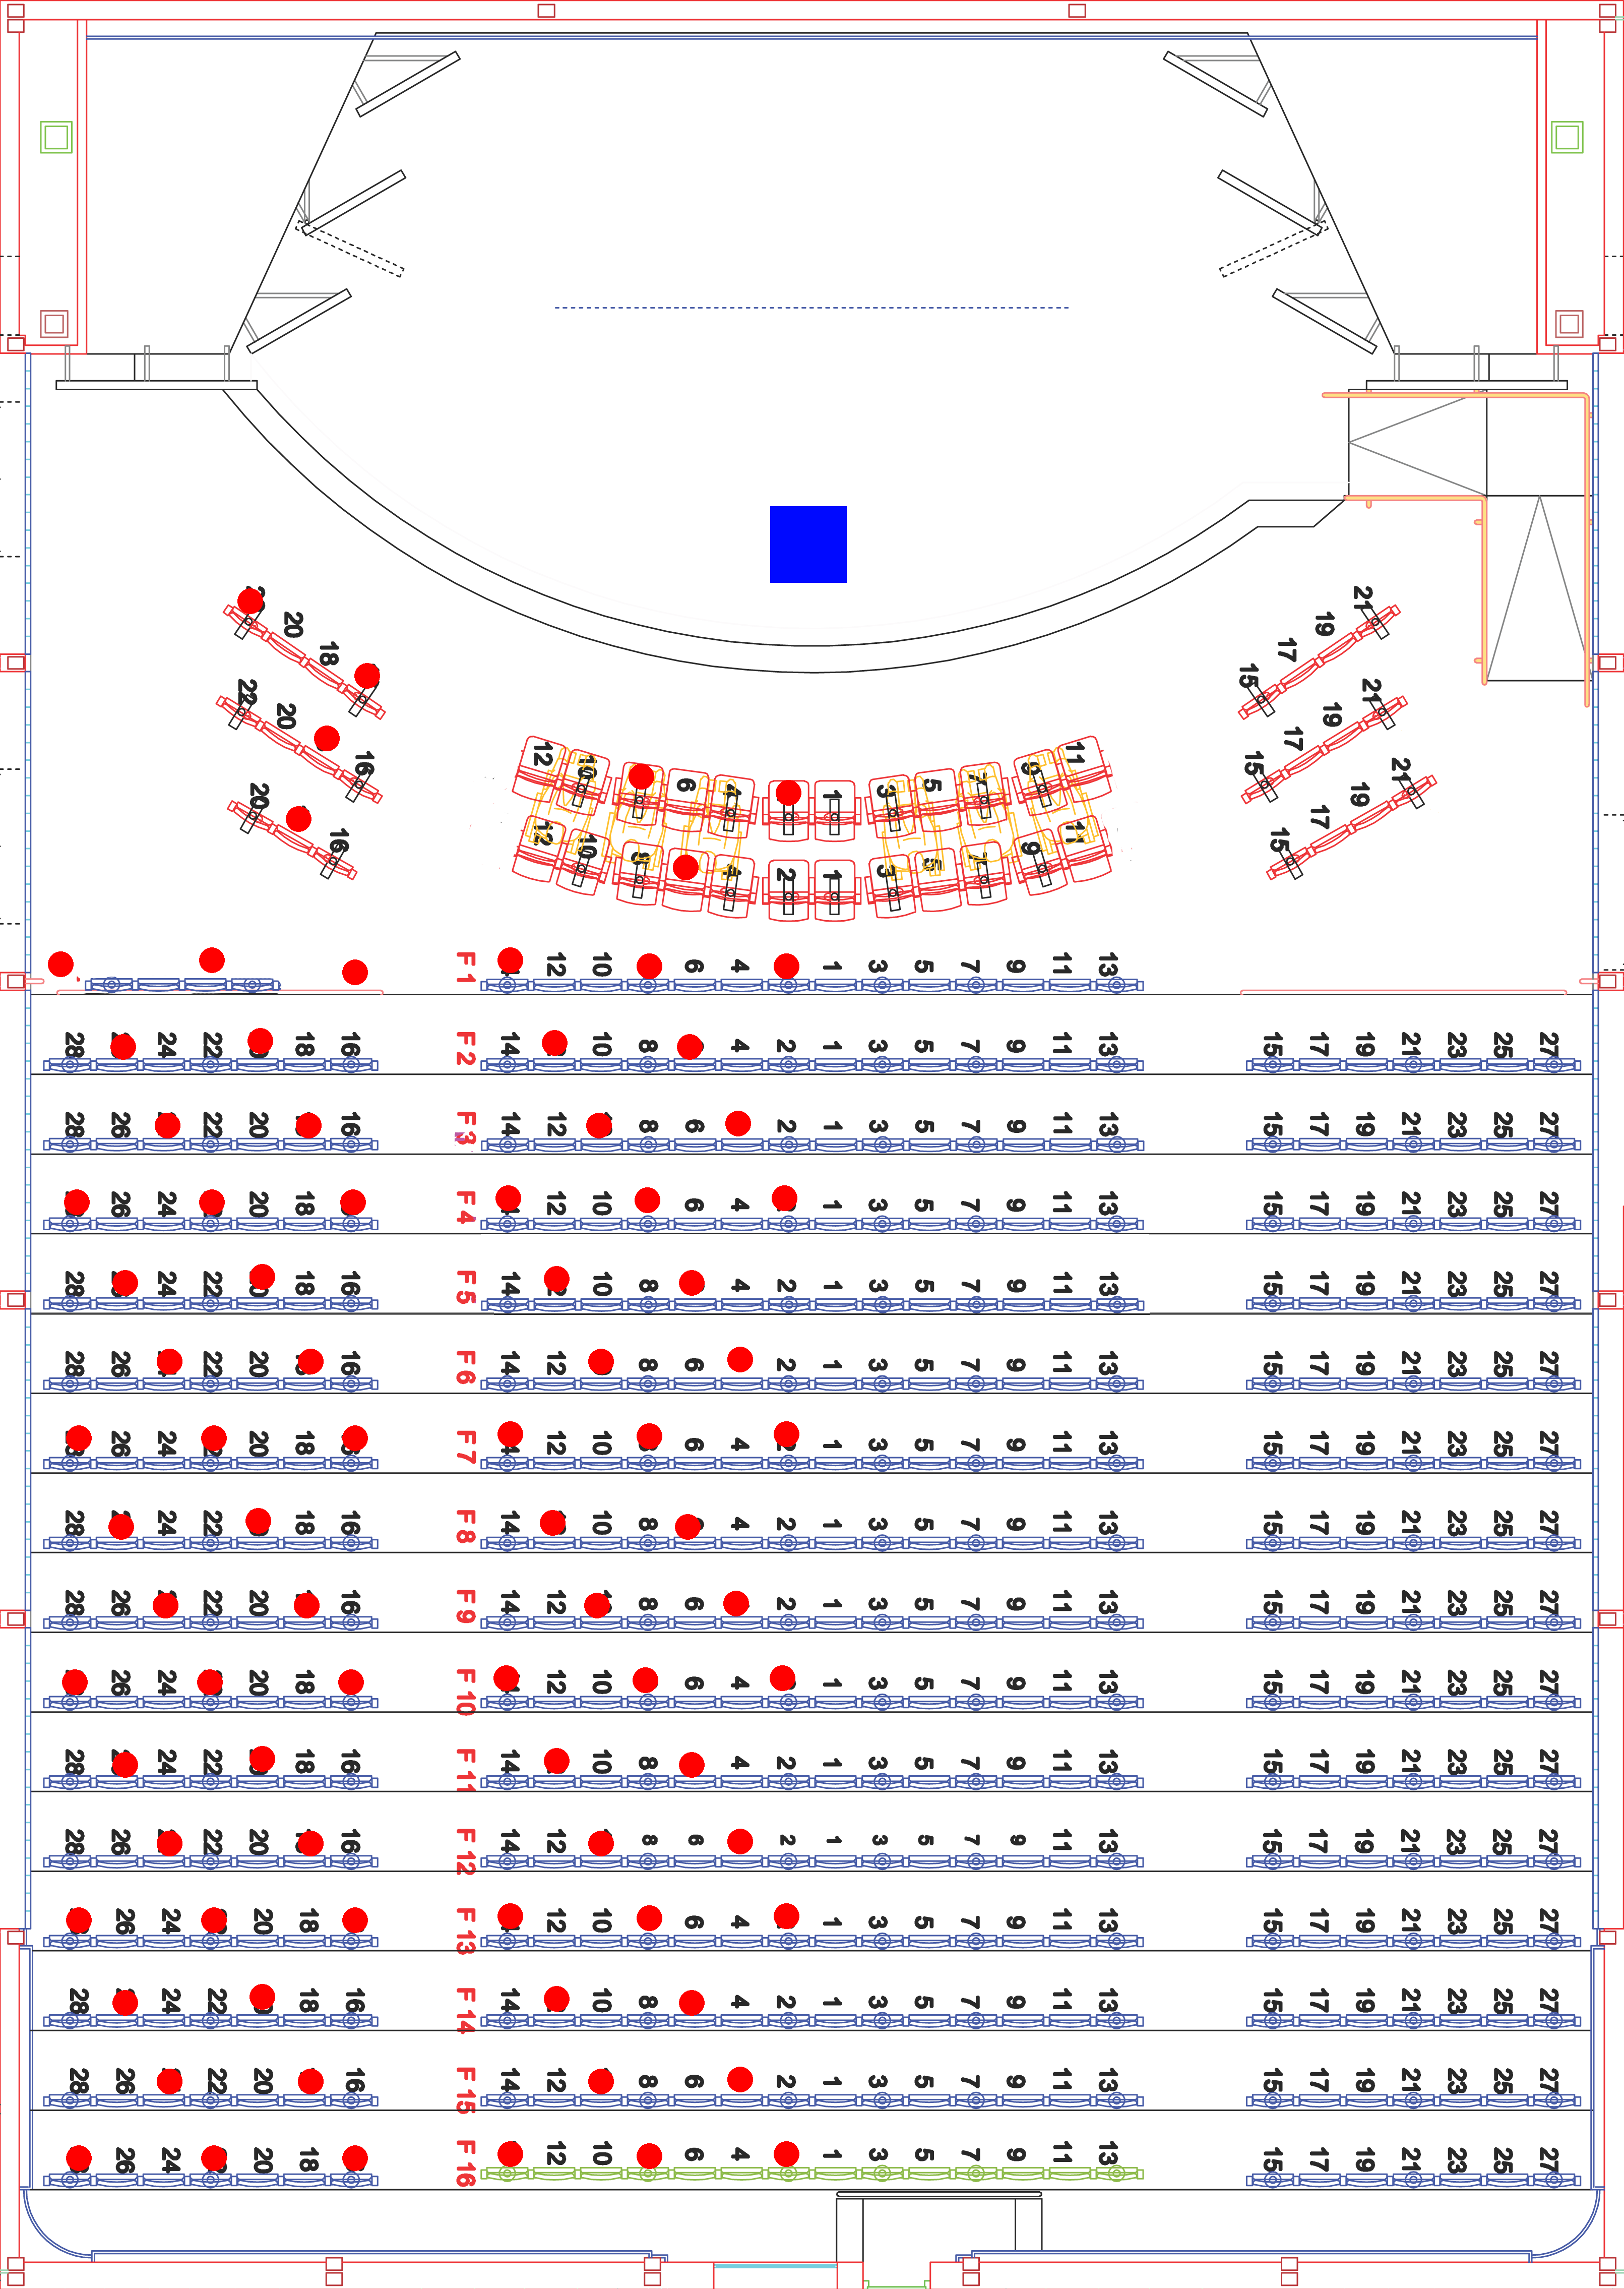
\includegraphics[scale=0.1]{../imagenes/auditorio_butacas_marcadas.png}
			    \centering
			    \caption{Distribución de las posiciones de grabación de las respuestas impulsivas. El cuadrado azul marca la posición de la fuente de sonido y los círculos rojos las posiciones de los micrófonos.}
			    \label{fig:butacasMarcadas}
	        \end{figure}

		    Como la toma de los datos se ha realizado en el transcurso de dos días, se ha optado por repetir las medidas en algunas posiciones. De esta forma se pretende obtener más información y asgurarnos de que la respuesta en dicha posición no varía en gran medida de un día para otro (por variaciones de temperatura, humedad, etc.). También se seleccionaron algunas posiciones de la parte impar del escenario. El motivo era para comprobar en la versión preliminar del test si nuestra hipótesis inical de la simetría de la sala era respaldada por las escuchas subjetivas de un pequeño número de participantes. Estas posiciones se encuentran en las posiciones extremas de la sala; es decir, las zonas más cercanas y lejanas al centro del escenario en la primera y última fila.

	    \subsection{Equipo utilizado para la toma de los datos}
	        Para la grabación de las respuestas impulsivas se ha utilizado el siguiente equipo:
	        \begin{itemize}
	            \item Ordenador portátil ASUS 2 con Windows 10 y software Dirac instalado.
	            \item Tarjeta de sonido MOTU UltraLite-mk3 Hybrid.
	            \item Amplificador de potencia Crown XLS 2002.
	            \item Fuente dodecaédrica AVM DO-12.
	            \item Micrófono ominidireccional AKG-CK92.
	            \item Micrófono bidireccional AKG-CK94.
	            \item Alargaderas y cableado necesario para el conexionado de los equipos.
	            \item trípodes y sujecciones para los micrófonos.
	        
	        \end{itemize}
	    
	        En la figura \ref{fig:equipos} se pueden observar imágenes sobre varios de dichos equipos, en la figura \ref{fig:control} se muestra cómo se organiza la zona de control para la realización de las medidas ubicada dentro del mismo salón de actos y en la figura \ref{fig:bloques1} se puede observar el diagrama de bloques de los equipos conectados para la toma de datos.
	    
	        \begin{figure}[H]
	            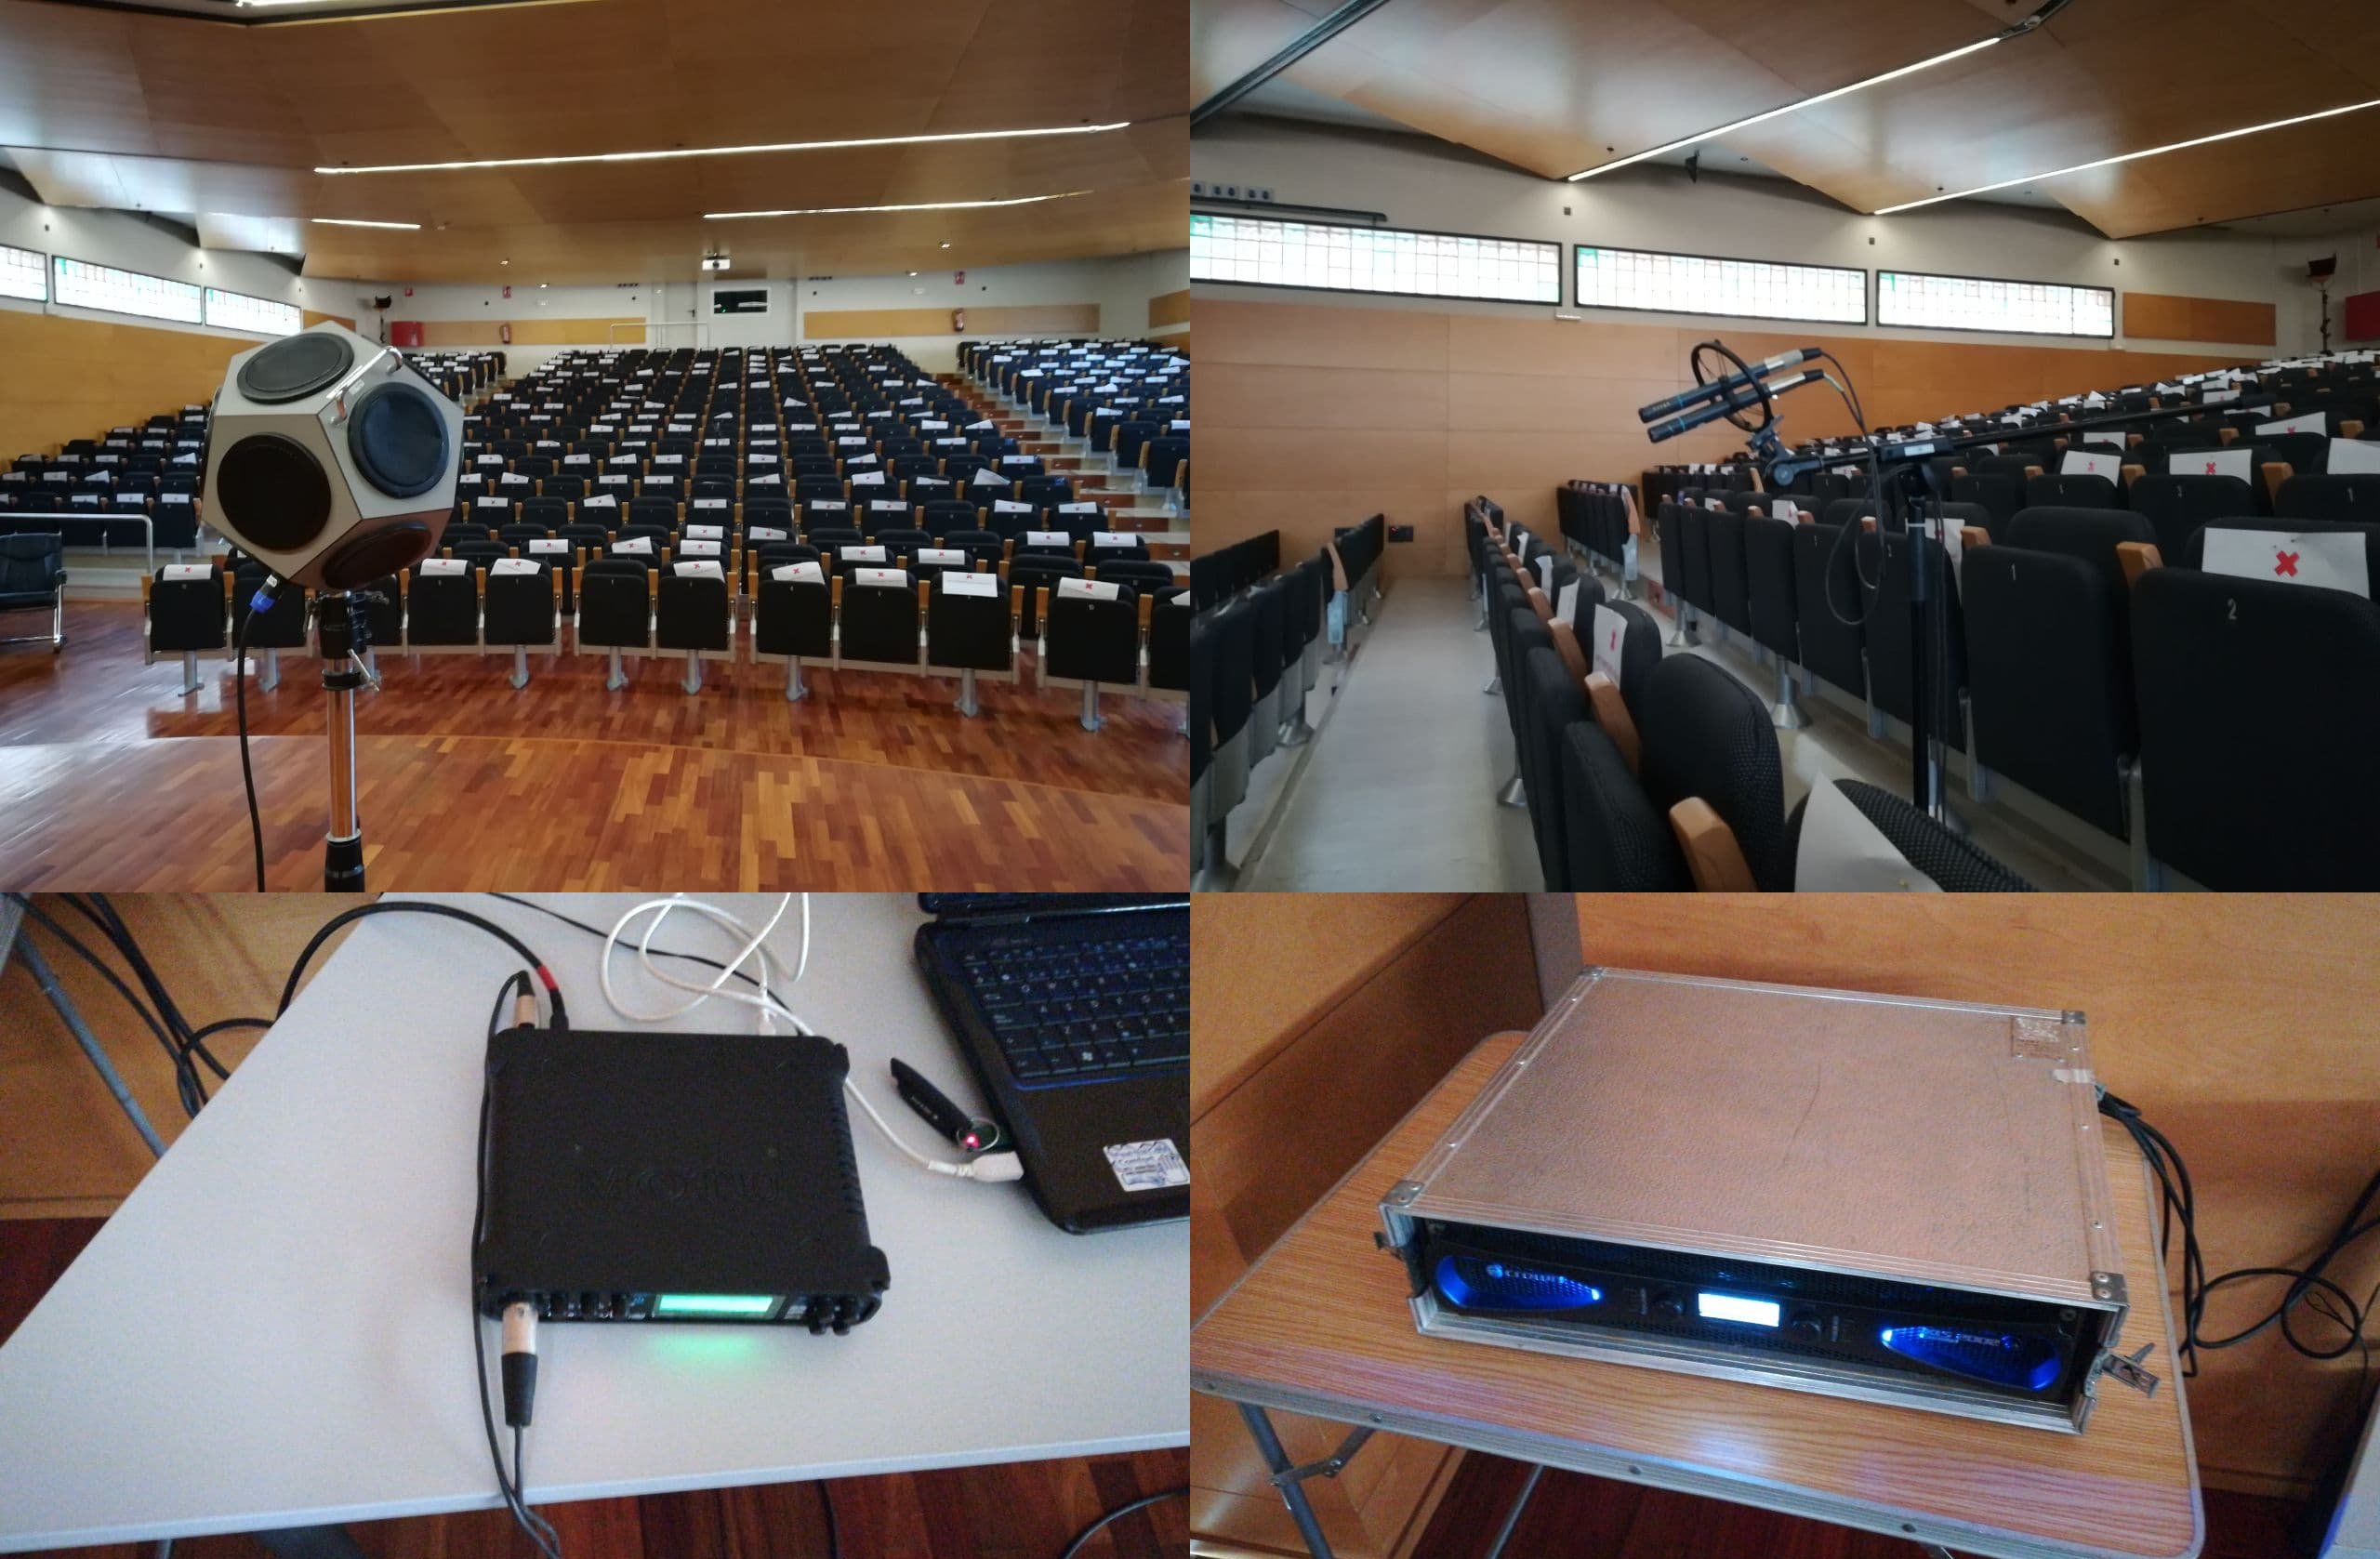
\includegraphics[scale=0.6]{../imagenes/equipos.jpg}
			    \centering
			    \caption{De izquierda a derecha y arriba a abajo: Fuente dodecaédrica, disposición de los micrófonos de medida, tarjeta de sonido MOTU y amplificador de potencia Crown.}
			    \label{fig:equipos}
	        \end{figure}
	    
	        \begin{figure}[H]
	            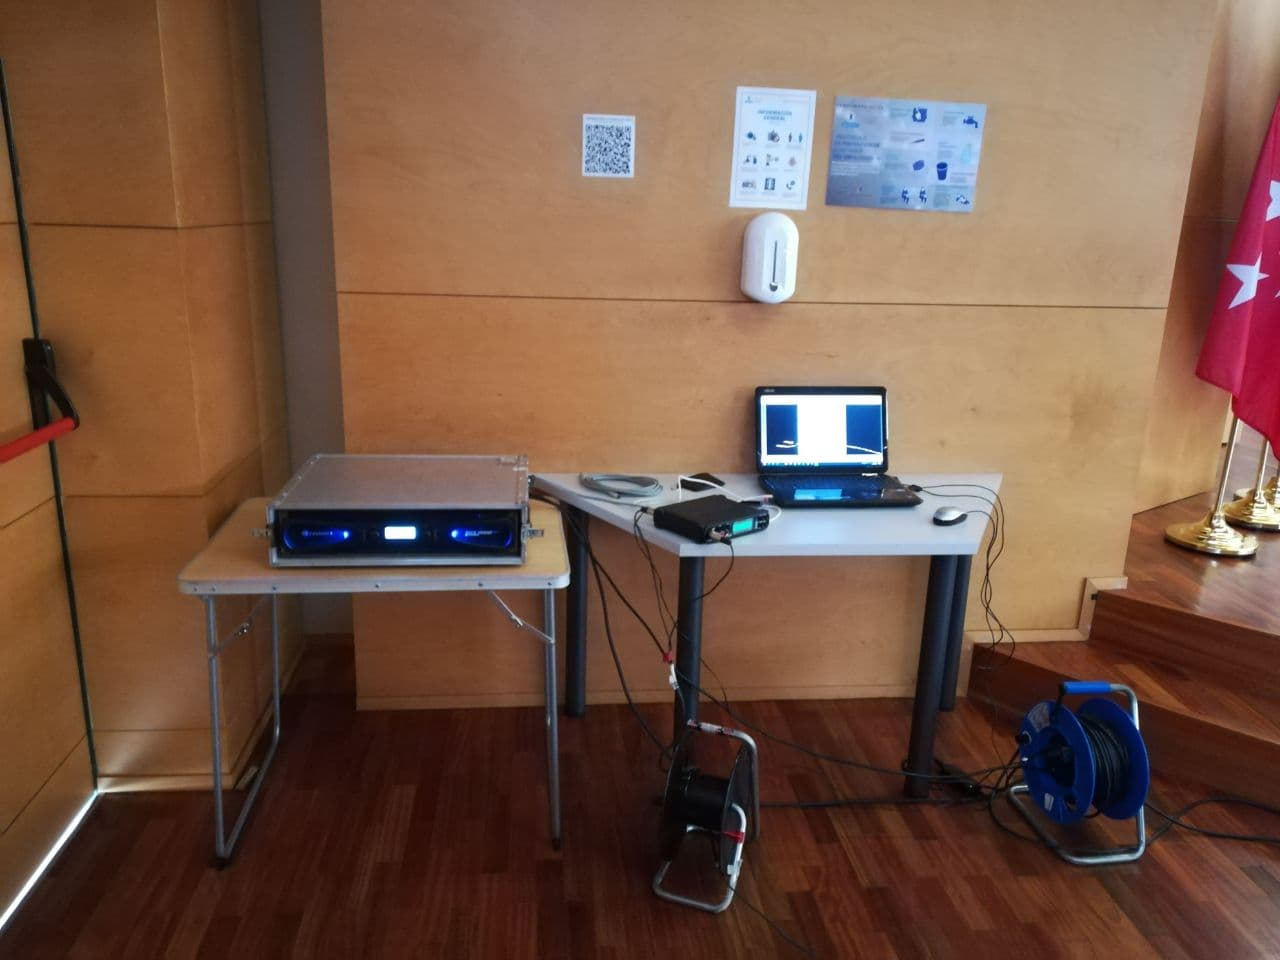
\includegraphics[scale=0.4]{../imagenes/control.jpg}
			    \centering
			    \caption{Disposición de la zona de control para la realización de las grabaciones.}
			    \label{fig:control}
	        \end{figure}
	        
	        \begin{figure}[H]
	            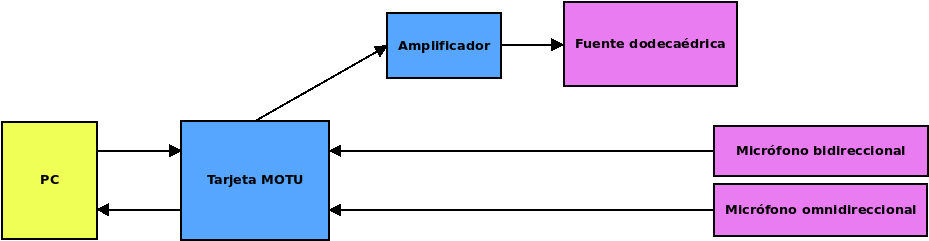
\includegraphics[scale=0.5]{../imagenes/diagrama_bloques1.png}
			    \centering
			    \caption{Diagrama de bloques utilizado para la primera toma de datos}
			    \label{fig:bloques1}
	        \end{figure}
	    
        \subsection{Metodología para la grabación de las respuestas al impulso}
            Una vez escogidas las posiciones de medida y conectados los equipos, se procede a realizar una medida de las condiciones atmosféricas. Más concretamente, se toma una medida de la temperatura y la humedad relativa presente en el recinto. En el día 2 de junio de 2021 (primer día de mediciones) se registró una temperatura de 27ºC y una humedad relativa del 34.5\% tanto al inicio como al fin de las medidas. El 9 de junio de 2021 (segundo día) se obtuvieron las mismas temperaturas y humedades relativas que el primer día.
        
            A continuación, se coloca la fuente dodecaédrica en el centro del escenario, que es el punto de referencia que se va utilizar para realizar las medidas; también se colocan ambos micrófonos en el trípode, a la altura que se correspondería con los oídos de una persona de ``altura media'', y se situa en la posición más lejana respecto de la fuente que se va a medir. Una vez situados, se enciende el amplificador, la tarjeta de sonido y el ordenador. Tras comprobar que el ordenador detecta correctamente la tarjeta de sonido, se inicia el programa ``Dirac''. En él, se accede a los parámetros de configuración de las medidas fijando las entradas y salidas de la tarjeta de sonido correspondientes. También se determina la señal con la que se van a obtener las respuestas al impulso. En nuestro caso, se opta por un barrido sinusoidal lineal desde los 20 Hz a los 20 kHz los  de algo más de cinco segundos de duración. Se opta por esta duración porque el tiempo de reverberación aproximado del salón de actos es de algo más de 1.2 segundos. Por este motivo, el barrido debe tener una duración de al menos el doble de duración y esta opción tiene margen suficiente.
        
            Una vez configurado el software, se realizan varias pruebas de la medida ajustando la ganancia del amplificador de forma que se obtiene una relación señal a ruido suficiente. Es en este mometno en el que se aprecia un ruido eléctrico debido al sistema de iluminación del auditorio y se apagan para minimizar dicho ruido. También se optó por apagar el sistema de climatización del auditorio. Para el calculo mediante la estimación del tiempo de reverberación T20, se requiere una relación señal a ruido de 35 dB en todas las bandas de frecuencia. Este ajuste se realiza teniendo especial precaución de que la fuente no empiece a distorsionar. Una vez ajustado el amplificador, se repite la medición con los micrófonos situados en la posición más cercana a la fuente para comprobar que los niveles recibidos no saturan.
        
            Con estas comprobaciones realizadas, se procede a la obtención de las respuestas impulsivas. Se comienza desde las filas más alejadas a la fuente y se va avanzando una fila cada vez que se concluye la anterior siguiendo los esquemas presentandos en el apartado de ``Numeración y selección de las posiciones de toma de datos''. Para cada posición, una vez concluidos los dos barridos que realiza el software, se comprueba que la relación señal a ruido en todas las bandas sea superior a 35dB, como se explicó anteriormente. Si se produce algún evento extraño durante la reproducción o se sospecha que la respuesta es errónea, se repite la grabación. Este procedimiento se repite en todas las posiciones a lo largo de las dos sesiones de medidas.
        
            Es importante remarcar que se aseguró de que los cables utilizados y la ganancia aplicada es la misma en ambas sesiones. También se repitieron medidas en algunas filas con el fin de comprobar posteriormente que las respuestas son indistinguibles por parte de los oyentes.
        
            Al  final del proceso de toma de datos, se obtuvieron un total de 100 archivos de audio en formato ``.wav'' con la respuesta al impulso obtenida en cada una de las posiciones.
            
            \section{Procesado de los datos - Auralizaciones}
                Una vez obtenidos los datos, se planteó la cuestión sobre qué tipo de audio sería más conveniente: si las respuestas al impulso o bien dichas respuestas convolucionadas con otros audios anecoicos (también conocido como audios \textit{auralizados}). En un primer momento se optó por la segunda opción por varios motivos.
        
                El primero es que las personas están más acostumbradas a escuchar, y por tanto comparar, sonidos de carácter más melódico que se alejan de las respuestas al impulso, las cuales son parecidas al producido por un disparo.
        
                Otro motivo es que este sistema permite escoger un tipo de sonido que se ajuste en buena medida al tipo de evento para los que la sala está pensada con la ventaja añadida de que no se necesita que dicho evento se realice en el momento de las grabaciones.
        
                El audio utilizado está obtenido de la página web de OpenAir de la universidad de York que incluye numerosos audios anecóicos de diferentes cateogrías y también respuestas impulsivas de diferente tipos de espacios grabados por todo el mundo. Particularmente, se escoge la grabación de una voz femenina haciendo una escala musical. Esto se corresponde con el uso principal del Salón de actos que consiste en conferencias y música de coro.
        
                Para la auralización se utiliza el software de Cycling74 ``MaxMSP'' junto con el plugin de la Universidad de Huddersfield, ``\textit{HISSTOOLS}''. Este programa permite realizar la convolución de la respuesta al impulso grabada con el audio anecoico de forma que se obtiene el audio auralizado que se desea. Para ello, se crea un pequeño script o ``\textit{patch}'' que realiza dicho procedimiento para todas las respuestas impulsivas previamente grabadas y se almacenan las convoluciones en una nueva carpeta de forma automática. Dicho \textit{patch} puede observarse en la siguiente figura \ref{fig:convolver_max}. Del mismo modo, se incluye una versión texto de dicho script en el Anexo XX.
                
                Por comodidad, se mantiene la misma numeración y terminología para los audios convolucionados que se había seguido para las grabaciones; siendo la única diferencia la carpeta donde se almacenan.
        
                \begin{figure}[H]
	                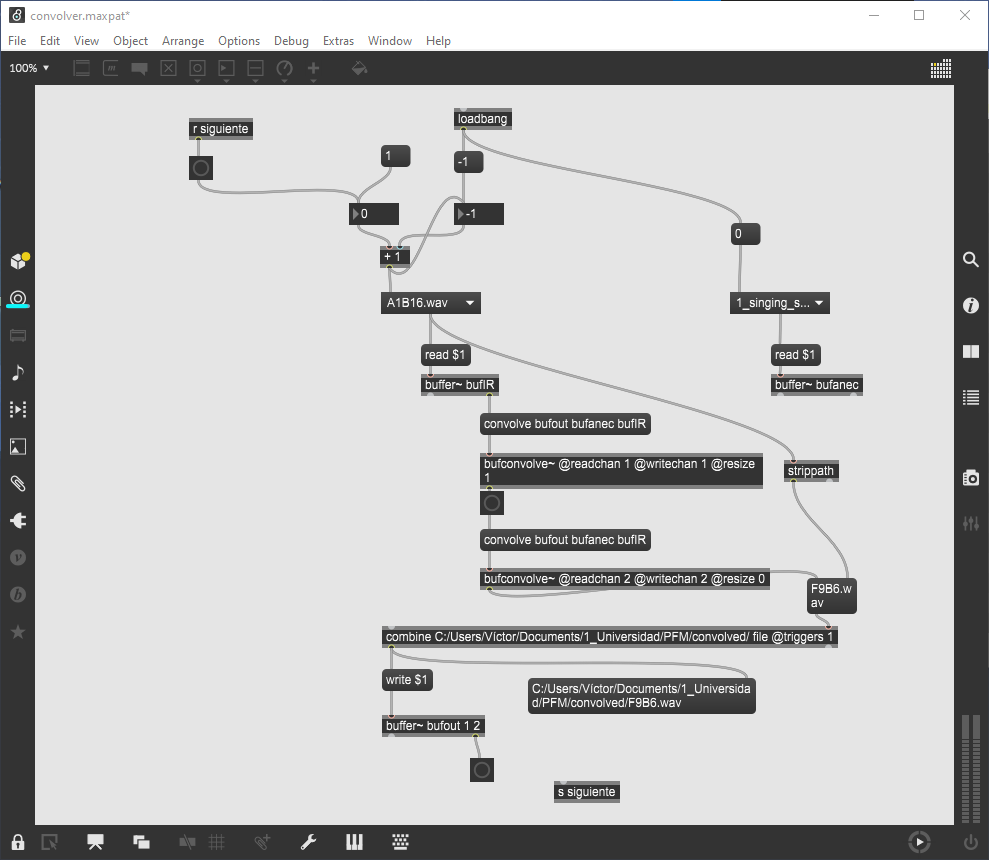
\includegraphics[scale=0.4]{../imagenes/convolver_max.png}
			        \centering
			        \caption{Patch en MaxMSP para la convolución de las respuestas impulsivas con el audio anecoico.}
			        \label{fig:convolver_max}
	            \end{figure}
        
                Al final este procesado no se realizó para la segunda toma de datos y, por consiguiente, en el test final. Esto se debe a que el proceso de auralización puede incluir una serie de variables aleatorias adicionales que pueden condicionar los resultados. Además, para la detección de diferencias perceptuales, que es el objetivo del proyecto, las respuestas al impulso tienen suficiente información acústica para realizar el proyecto. Este sistema cuenta con la ventaja adicional de que la duración de las señales es menor, por lo que se reduce la posibilidad de que los participantes experimenten fatiga auditiva durante la realización del test.
            
    \section{Segunda toma de datos}
        Durante fases posteriores del proyecto, se localizó un error en el procesado de las señales que las hicieron inservibles para el propósito de nuestro proyecto. Debido a esto, y a la adquisición de unos micrófonos biaurales, se decidió realizar una nueva toma de datos con las que realizar el test subjetivo final.
        
        
       \subsection{Numeración y selección de las butacas en la segunda toma de datos}
            Para la segunda toma de datos, se siguió la misma numeración que la vez anterior. Es decir, para las butacas normales, se sigue la estructura ``FxBy'' siendo ``x'' e ``y'' el número de fila y de butaca respectivamente tal y como ya se mostró en el apartado de la primera toma de datos.
                
            Del mismo modo, para las tres filas más próximas al escenario, la numeración utilizada es de la forma ``AxBy'' en la que, de nuevo, ``x'' e ``y'' tienen el mismo significado.\newline
                
            La selección de las posiciones de grabación también sigue el mismo criterio aplicado la otra vez: se selecciona una de cada tres butacas de la mitad derecha del escenario. En la fila siguiente se desplaza la primera butaca una posición a la derecha. Puede volverse a consultar la figura \ref{fig:butacasMarcadas} para observar todas las posiciones de grabación.
                
            Al contrario que la otra vez, esta vez no se han seleccionado las posiciones extremas del lado izquierdo ya que, tras el experimento previo, se vio que los participantes podrían distinguirlos perfectamente. Del mismo modo, como la toma de datos se realizó en un único día, no se repitieron medidas en ninguna posición, aunque tampoco sería necesario porque ya se observó tras el primer test que los oyentes eran incapaces de distinguirlos entre sí. Esto puede comprobarse en el apartado de ``Análisis del test previo'' dentro del capítulo ``Análisis estadístico''.
                
                
        \subsection{Equipo utilizado para la segunda toma de datos}
            Para esta nueva toma de datos, la principal diferencia en torno al equipo utilizado se encuentra en los micrófonos utilizados. En este caso, se utilizaron unos micrófonos biaurales ``Roland CS-10EM''. Estos micrófonos tienen la particularidad de que tienen la forma de auriculares \textit{in-ear} y se conectan mediante un conector mini-jack estéreo. Estos micrófonos necesitan que se les suministe una alimentación de entre 2 y 5 Voltios, algo que no es posible en la tarjeta de sonido MOTU que se utilizó en la anterior toma de datos. Por este motivo, se realiza la grabación de las señales a través de una grabadora de audio externa que permite aplicar dicha alimentación. Para nuestro caso, se ha optado por una ``Yamaha pr7''. En la figura \ref{fig:microsBi} pueden observarse tanto los micrófonos como la grabadora.
                
            \begin{figure}[H]
                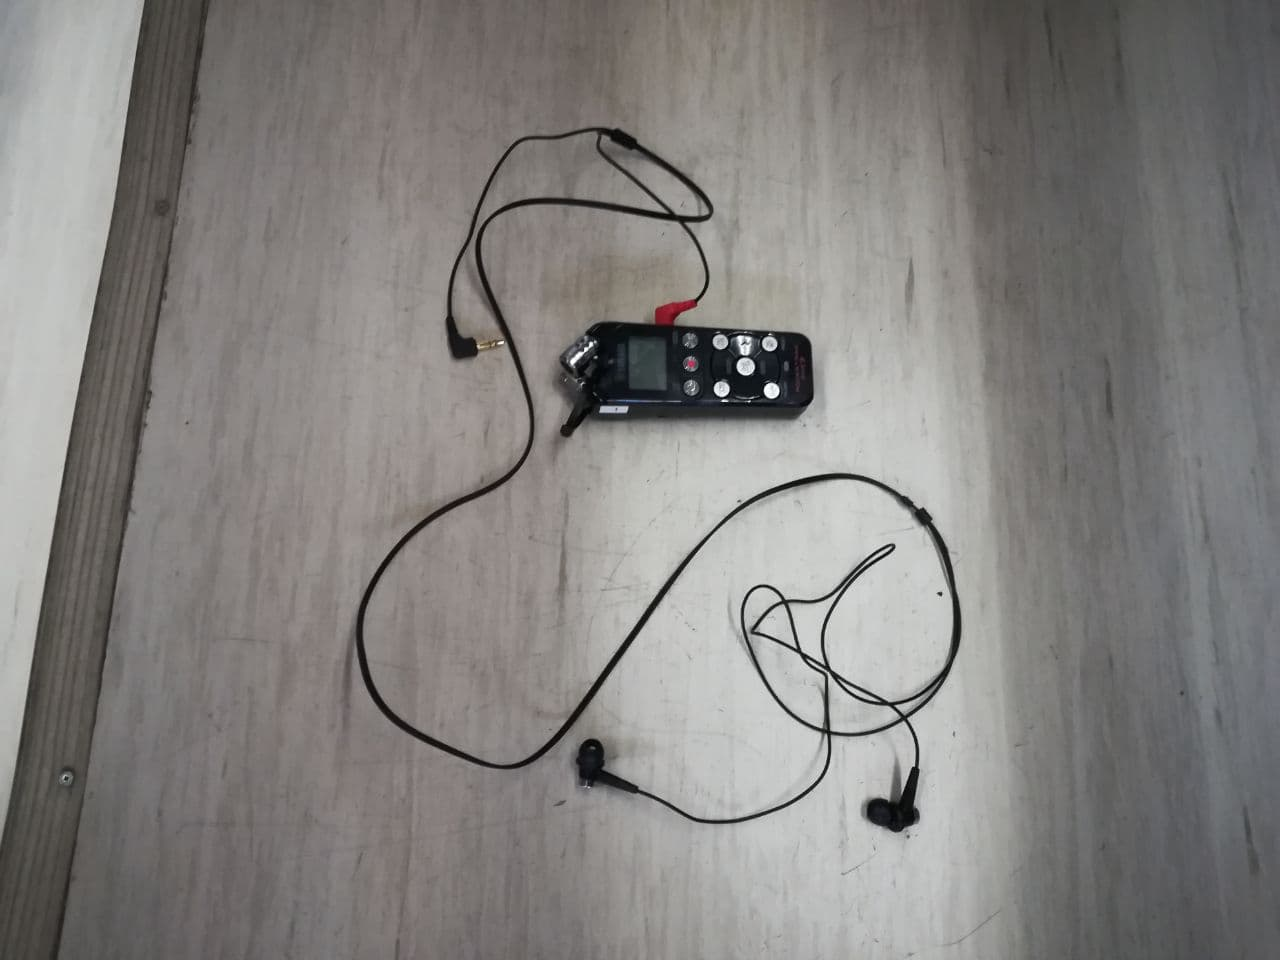
\includegraphics[scale=0.3]{../imagenes/MicroBi.jpg}
                \centering
                \caption{Micrófonos biaurales Roland y grabadora Yamaha utilizada para la grabación de las respuestas.}
                \label{fig:microsBi}
            \end{figure}
                
            La tarjeta de sonido se sigue utilizando para controlar la fuente de sonido dodecaédrica al igual que la vez anterior.
                
            A modo de resumen, se adjunta una nueva lista con todo el equipamiento utilizado para la grabación de las respuestas:
                
            \begin{itemize}
                \item Ordenador portátil ASUS 2 con Windows 10 y software Dirac instalado.
	            \item Tarjeta de sonido MOTU UltraLite-mk3 Hybrid.
	            \item Amplificador de potencia Crown XLS 2002.
	            \item Fuente dodecaédrica AVM DO-12.
	            \item Alargaderas y cableado necesario para el conexionado de los equipos.
	            \item Micrófonos biaurales Roland CS-10EM.
	            \item Grabadora portátil Yamaha pr7.
            \end{itemize}
                
            En la figura \ref{fig:equipos}, ya presentada anteriormente, pueden observarse imágenes de algunos de los equipos ya mencionados y en la figura \ref{fig:bloques2} X el nuevo diagráma de bloques para esta toma de datos.
            
            \begin{figure}
	            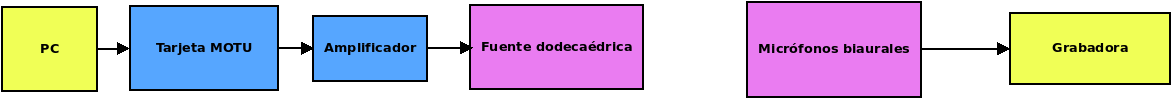
\includegraphics[scale=0.47]{../imagenes/diagrama_bloques2.png}
			    \centering
			    \caption{Diagrama de bloques utilizado para la segunda toma de datos}
			    \label{fig:bloques2}
	        \end{figure}
            
            
                
        \subsection{Metodología para la grabación de las respuestas al impulso}
            La metodología seguida para la grabación de esta tanda de señales es muy similar a la ya comentada anteriormente.
                
            En primer lugar, se procede a hacer una escucha de las fuentes de ruido que se aprecian dentro del espacio. De esta forma, se localizó un ruido eléctrico debido a la iluminación del salón de actos. Este ruido desaparecía al apagar las luces, por lo que se optó por dejarlas apagadas durante las grabaciones, ya que desde los ventanales entraba luz suficiente para poder realizar el trabajo. Del mismo modo, se localizó un ruido esporádico procedente de uno de los altavoces montados en el escenario. A primera vista parecía debido a algún problema de contacto, pero no había forma de asegurarse. Por suerte, era de un nivel aceptable y su duración era muy escasa de forma que no se percibía mientras se reproducían los barridos.
                
            Una vez analizadas las diferentes fuentes de ruido, se procede a calibrar el sistema de forma que la relación señal a ruido en las posiciones más lejanas respecto de la fuente sean aceptables (mayor o igual a 35dB) y que ni la fuente ni los micrófonos saturaran en ningún momento.
                
            Una vez hecha esta comprobación, se comenzó con las grabaciones. El orden seguido fue desde las filas más alejadas a la fuente a las más cercanas. La persona encargada de ser sujeto de las medidas se colocaba los auriculares y se sentaba en la butaca que correspondía como se aprecia en la figura \ref{fig:Nico}. Una vez colocado, se comenzaba la reproducción de cuatro rondas de barridos frecuenciales de 20Hz a 20kHz. El sujeto debía iniciar manualmente la grabación una vez terminaba de reproducirse el primer barrido y finalizarla una vez terminaba el tercer barrido. Una vez realizada la grabación, se comprobaba que se había grabado correctamente y se pasaba a la siguiente posición. 
                
            \begin{figure}[H]
                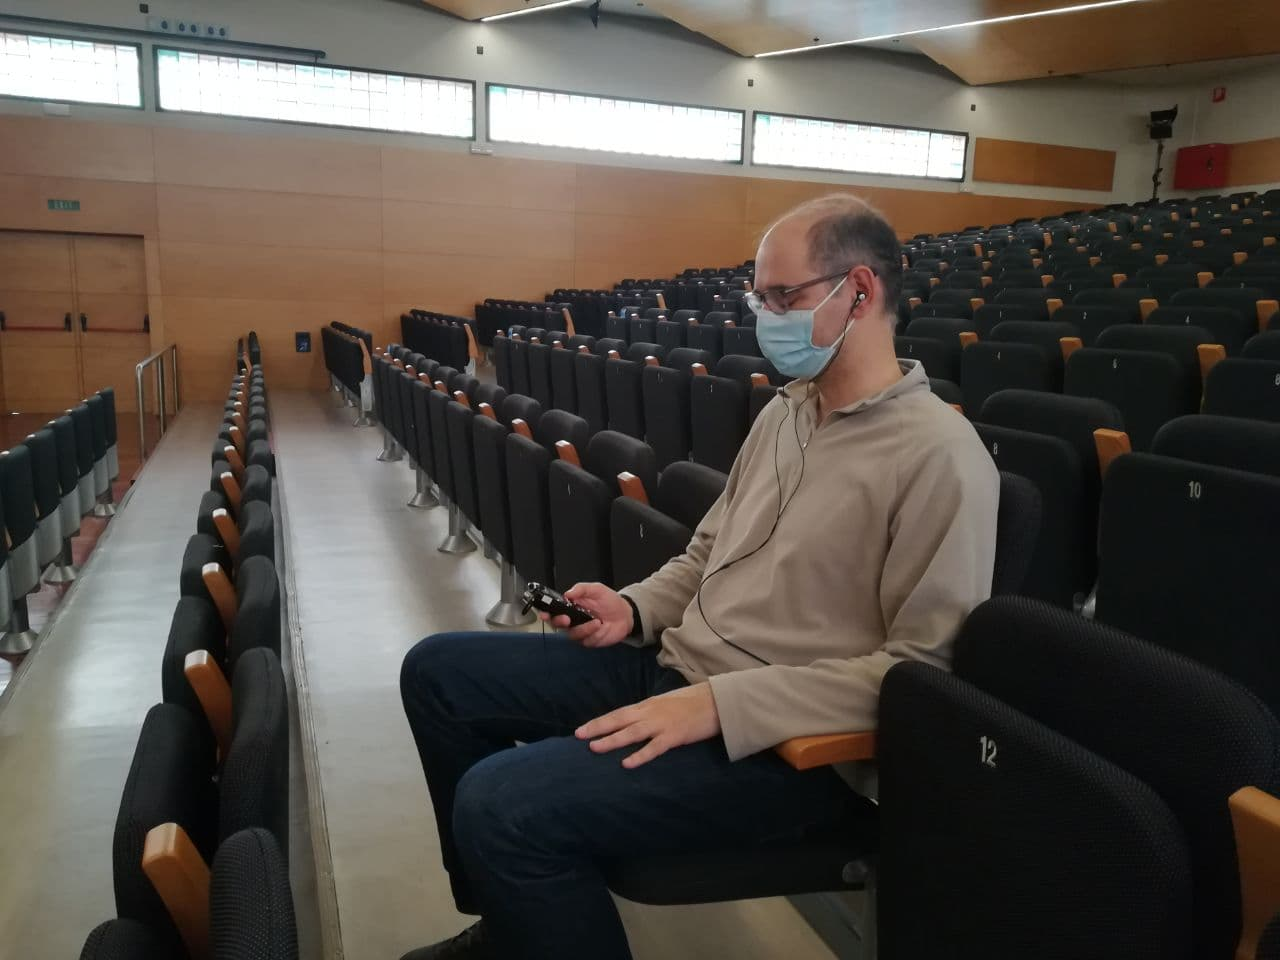
\includegraphics[scale=0.3]{../imagenes/Nico.jpg}
                \centering
                \caption{Ejemplo de la disposición del sujeto para la grabación de las señales. Los micrófonos se encuentran en sus oídos.}
                \label{fig:Nico}
            \end{figure}
                
            En total se obtuvieron unas 83 grabaciones que, a continuación, se procesaban en el mismo ordenador utilizando el software Dirac con el fin de obtener las respuestas al impulso. Para ello, se utiliza el mismo menú utilizado en la primera toma de datos, pero esta vez, en vez de realizar una grabación, se importa la señal ya grabada y se le pide al programa que calcule la respuesta al impulso utilizando como señal de referencia la misma utilizada en la reproducción de la fuente. De forma que el programa genera al final un archivo como el que se observa en la figura X.
            
        \subsection{Procesado de los datos}
            Para esta seguna toma de datos, se ha decidido no realizar el proceso de auralización de las señales con los audios anecoicos. Esto se debe a que el proceso de auralización no es perfecto y que, al final, a pesar de que son señales más ``habituales'' para los participantes, no nos aportan nada que no se pueda conseguir reproduciendo diréctamente las respuestas al impulso.
            
            A nivel de procesado para esta parte, sólo se ha recortado la duración del fichero de audio para ajustarlo a la duración de la señal y no hacer que los oyentes escucharan largos tramos de silencio. En ningún momento se modifican las ganancias de las señales para evitar que la información acústica pueda quedar modificada respecto de los valores de grabación. El ajuste de volumen para que sea cómodo se realizará en el test mediante los ajustes de volumen del sistema operativo.
            
    \section{Medida de distancias clave}
        Para un correcto análisis de los resultados, es necesario realizar una serie de medidas en el auditorio. Esto nos permite, más adelante, poder organizar los resultados en función de diferentes referencias y ver si existe alguna relación entre ellas. En nuestro caso, hemos considerado como importantes las distancias de la fuente dodecaédrica a la primera butaca, la distancia entre filas, entre butacas, el ancho del pasillo, entre otras. Las distancias que se midieron pueden observarse en la figura \ref{fig:distancias} y el resto pueden obtenerse a partir de las que ahí vienen reflejadas.
        
        \begin{figure}
                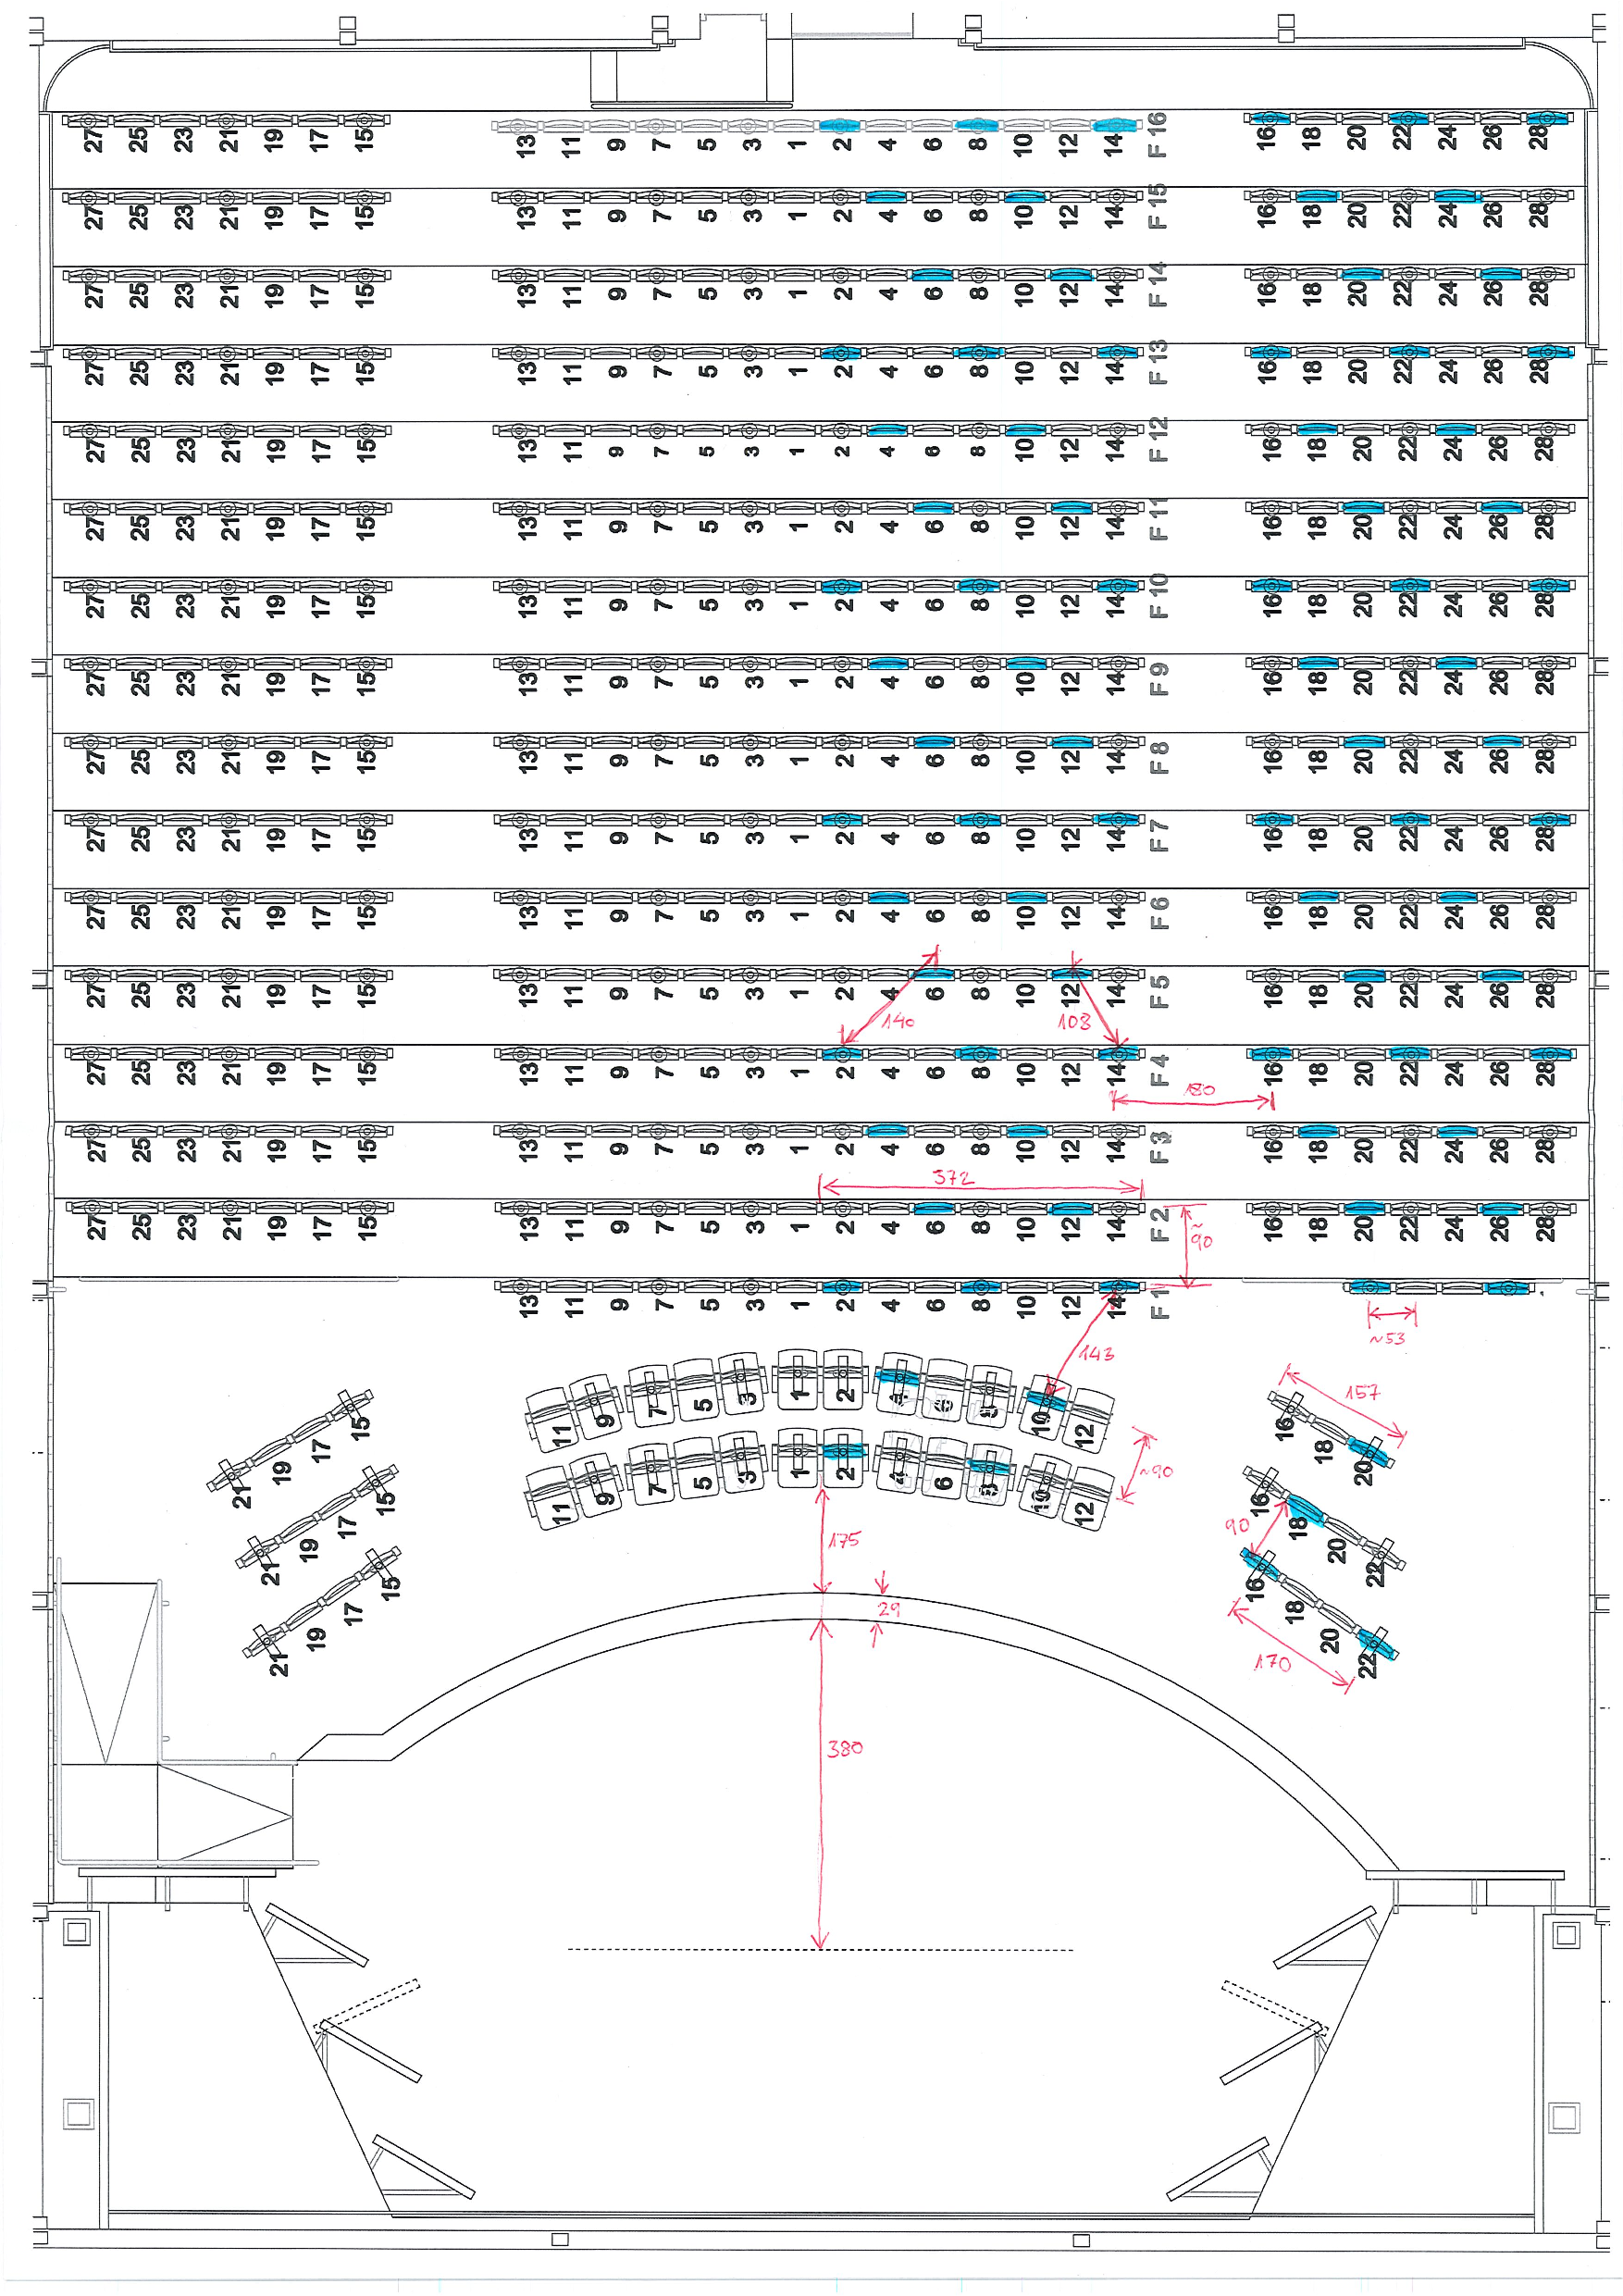
\includegraphics[scale=0.4]{../imagenes/AuditorioMedidasButacas.pdf}
                \centering
                \caption{Medidas de distancias tomadas dentro del auditorio.}
                \label{fig:distancias}
            \end{figure}
    
    \chapter{Desarrollo de la aplicación del test subjetivo.}
        En este capítulo se explican las herramientas y lenguajes utilizados para la creación de la aplicación de escritorio con la que se realizan posteriormente los test subjetivos de audio necesarios para el proyecto. Así mismo, se explica el algoritmo utilizado y las diferentes versiones utilizadas para la creación de la interfaz de usuario.
        
        \section{Lenguajes y programas utilizados}
            Para el desarrollo de la aplicación, se ha optado por utilizar el lenguaje de programación Python3. Este lenguaje tiene la ventaja de que incluye numerosas librerías que permiten trabajar con interfaces gráficas con las que los participantes de los test puedan interactuar de forma sencilla. Para nuestro caso particular, se ha optado por utilizar la librería del entorno gráfico GTK (la librería se llama \textit{PyGObject}\footnote{https://pygobject.readthedocs.io/en/latest/}) que es una de las más utilizadas en entornos Linux, aunque también puede utilizarse en entornos de Windows o Mac.
            
            Para el diseño de la interfaz, se podría haber codificado diréctamente en lenguaje python. No obstante, se ha utilizado el programa Glade que permite utilizar un entorno gráfico para la creación de todos los elementos de la interfaz. Con dicho programa se obtiene un fichero XML con extensión ``.glade'' que es el que el \textit{script} de Python lee y con el que se genera la interfaz que el usuario utiliza. En la figura \ref{fig:gladeInic} se puede observar la pantalla de inicio de dicho programa. 
            
            \begin{figure}
                \begin{center}
                    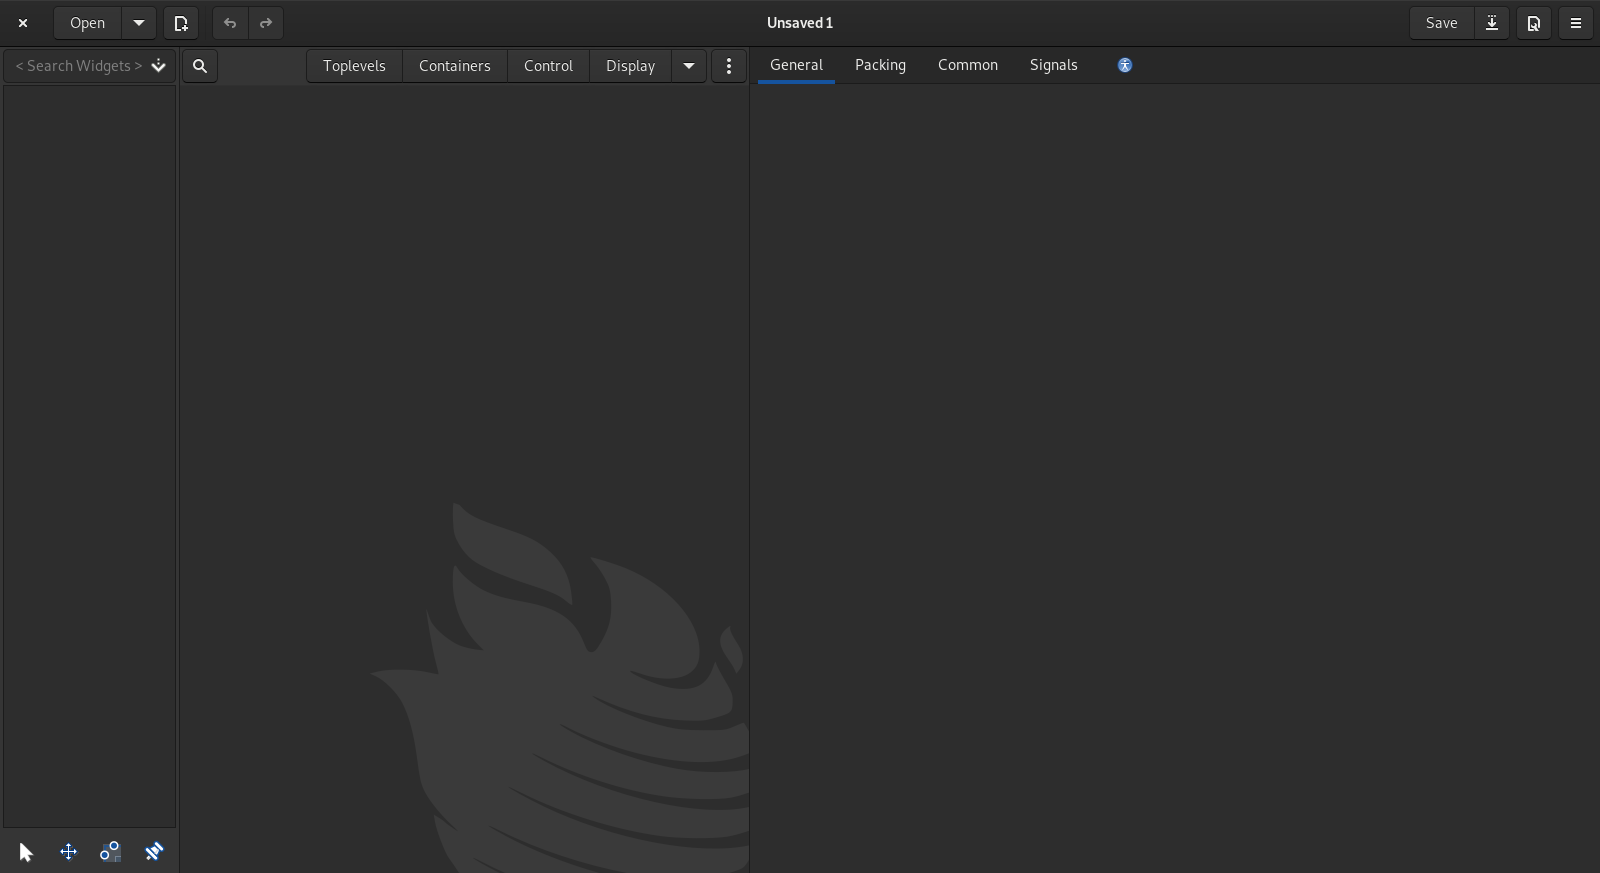
\includegraphics[scale=.2]{../imagenes/gladeInicio.png}
                    \caption{Ventana de inicio del programa \textit{Glade}.}
                    \label{fig:gladeInic}
                \end{center}
            \end{figure}
            
           \newpage

           Para la codificación de los scripts de Python se ha utilizado el programa ``\textit{Gnome Builder}''; un entorno de aplicaciones que incluye todas las herramientas para depurar, compilar y ejecutar los scripts dentro del mismo espacio. Al igual que con \textit{Glade}, el programa es gratuito de código abierto. En la figura \ref{fig:builderIni} se encuentra una captura de la interfaz del programa.
           
            \begin{figure}[H]
                \begin{center}
                    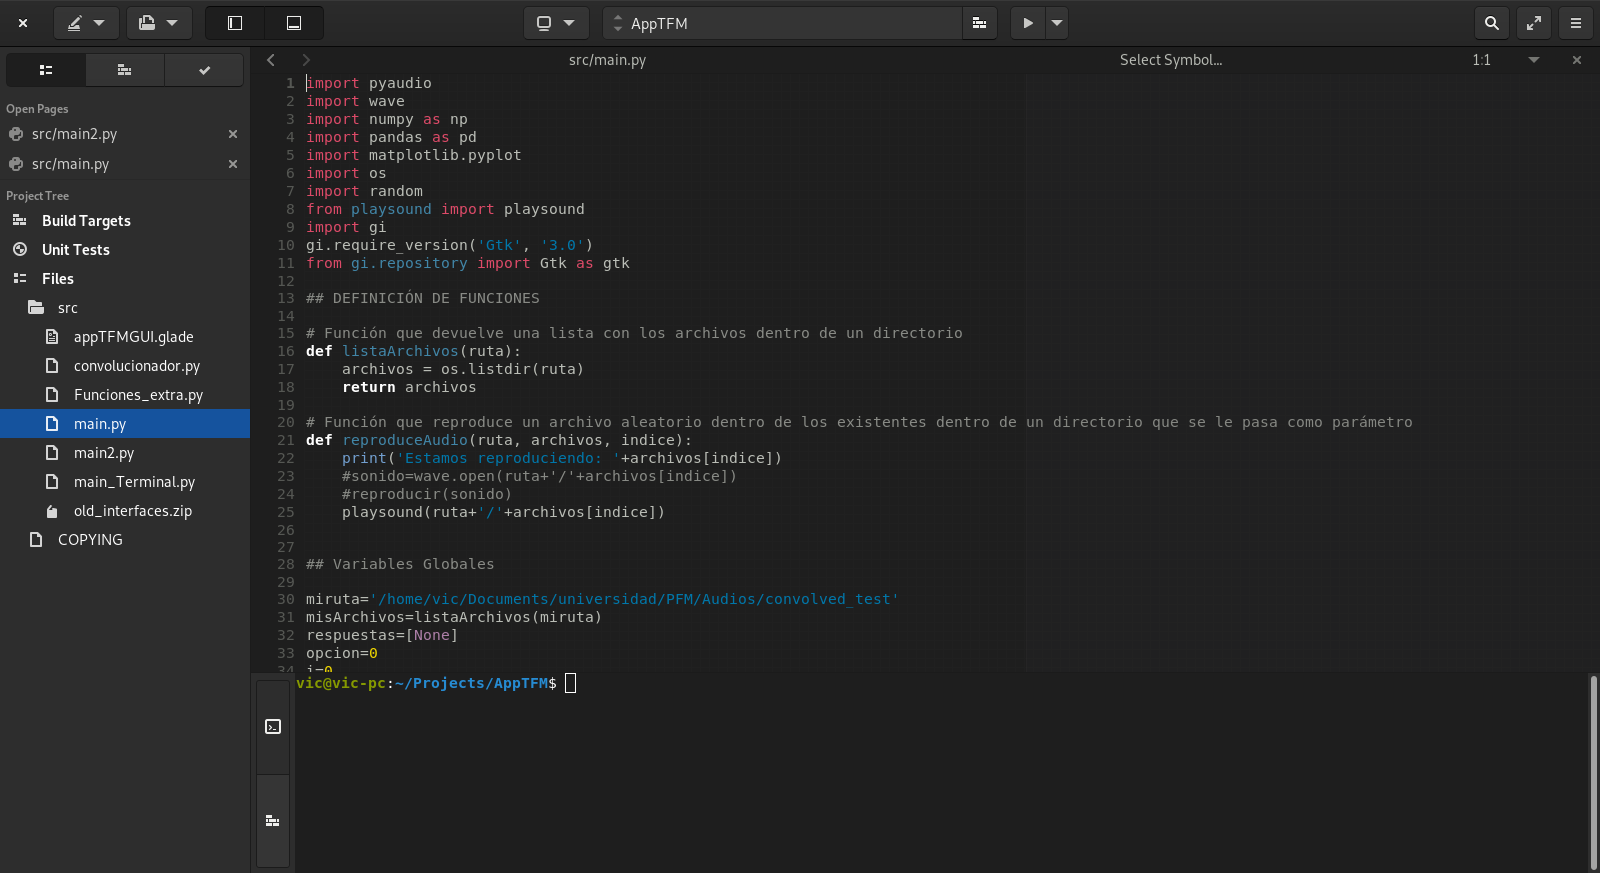
\includegraphics[scale=.2]{../imagenes/builderIni.png}
                    \caption{Captura del programa \textit{Gnome Builder}.}
                    \label{fig:builderIni}
                \end{center}
            \end{figure}
            
        \section{Características de la interfaz de usuario}
            Como se ha comentado en el apartado anterior, la interfaz de usuario se ha diseñado utilizando el programa ``\textit{Glade}''. Desde un principio, se ha querido diseñar una interfaz que sea lo más simple posible, no sólo por facilidad para realizarla, sino para que las personas participantes puedan centrarse exclusivamente en los aspectos del test y hacer que su uso no suponga ninguna dificultad.  
            
            En una primera instancia se decidió generar una interfaz en la que los elementos principales fueran dos botones con los que el usuario pudiera escoger cuál de los audios quería reproducir. Las respuestas se recogerían en dos casillas, o \textit{toggles}. También se incluyó un botón en la parte inferior para enviar cada una de las respuestas. En la parte superior se incluye un texto que indica el número de pregunta por la que va el test. Todos estos elementos se pueden observar en la figura \ref{fig:uiIni}.
            
            \begin{figure}[H]
                \begin{center}
                    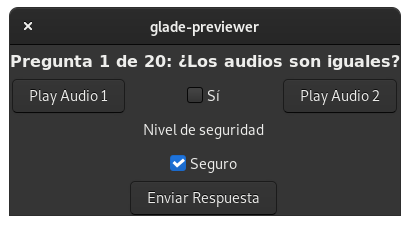
\includegraphics[scale=.6]{../imagenes/uiIni.png}
                    \caption{Versión inicial de la interfaz de usuario.}
                    \label{fig:uiIni}
                \end{center}
            \end{figure}
            
            Esta configuración es la que se utiliza en el test previo. Al finalizar dicho test, se les pidió a los participantes que propongan diferentes mejoras para perfeccionar la interfaz de usuario. Entre ellas, las más habituales consistieron en la sustitución de los \textit{toggles} por elementos más grandes al estilo de \textit{switches} o interruptores y la actualización de la posición de dichos elementos a su estado inicial entre cada una de las preguntas.
            Atendiendo a estas propuestas, se modifica la interfaz con el resultado que se muestra en la figura \ref{fig:uiFin}.
            
            \begin{figure}
                \begin{center}
                    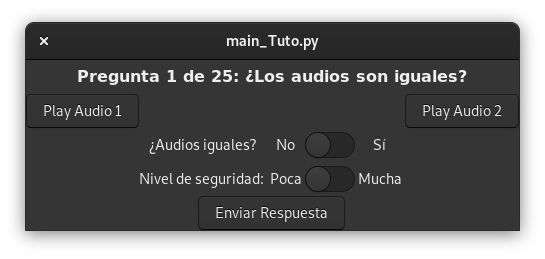
\includegraphics[scale=.6]{../imagenes/interFin.png}
                    \caption{Versión inicial de la interfaz de usuario.}
                    \label{fig:uiFin}
                \end{center}
            \end{figure}
            
        \section{Codificación del script en Python}            
            El procedimiento seguido para la codificación de la aplicación ha sido gradual. En primer lugar se han diseñado diferentes métodos y funciones que se apliquen diréctamente desde la consola. De esta forma, se comprueba que el algoritmo funciona correctamente y que se extraen los resultados en el formato deseado.
            
            Una vez, se ha comprobado que este \textit{script} funciona, se modifica el mismo haciendo que las diferentes funciones sean llamadas por los diferentes elementos de la interfaz de usuario ya creada y que se referencian dentro del código de Python.
            
            Durante todo el proceso, se realizaron consultas a la documentación de la API de Python para GTK\footnote{https://python-gtk-3-tutorial.readthedocs.io/en/latest/} y de las diferentes librerías necesarias para el desarrollo de la aplicación. Varios ejemplos de estas librerías son:
            \begin{itemize}
                \item \textbf{numpy}\footnote{https://numpy.org/}: para el trabajo con matrices al estilo de programas como \textit{Matlab}.
                \item \textbf{pandas}\footnote{https://pandas.pydata.org/}: para la edición y creación de estructuras de datos.
                \item \textbf{os}\footnote{https://docs.python.org/3/library/os.html}: para la navegación dentro de sistemas de ficheros del sistema operativo.
                \item \textbf{gi}\footnote{https://pygobject.readthedocs.io/en/latest/guide/api/api.html}: para el manejo de los elementos gráficos y la gestión de sus señales.
            \end{itemize}
            
            Por último durante el periodo de tiempo entre los dos tests subjetivos de audio se añadió la funcionalidad que permitía reproducir los dos audios pulsando las teclas ``1'' y ``2'' del teclado respectivamente sin necesidad de utilizar el ratón. Esta funcionalidad se incorporó como sugerencia por parte de varias de las personas participantes que comunicaron las dificultades de escuchar los audios con los ojos cerrados (decisión personal) al tener que pinchar los botones con el ratón del ordenador.
            
            \subsection{Estructura del código}
                El código de Python se encuentra dividido en diferentes partes:
                En primer lugar, la zona donde se importan las diferentes librerías para el correcto funcionamiento del script. Aquí se incluyen las que permiten reproducir los diferentes audios, manejar información, navegar por el sistema de archivos del ordenador, la interfaz gráfica, etc.
                
                A continuación, se encuentra una zona donde se definen diferentes funciones que serán usadas repetidamente a lo largo del \textit{script}. 
                
                Después, se definen algunas variables globales necesarias y da comienzo la clase \textit{Main} de la aplicación. En ella, se inicializan las referencias a los diferentes elementos de la interfaz gráfica con las que los usuarios interactúan y se establecen qué funciones se llaman en función de las señales que manejan. Estas funciones se definen en último lugar a continuación de dichas inicializaciones. En el anexo X se puede leer el código en su totalidad.
    
    \chapter{Realización de los test subjetivos de audio}
        Como ya se comentó en el capítulo de ``Introducción'', el objetivo del proyecto es el de analizar las diferencias perceptuales que se obtienen al escuchar las respuestas al impulso obtenidas al modificar la posición de escucha o recepción dentro de un determinado espacio.
        
        Para simplificar la toma de datos del estudio, se parte de la premisa de que los oyentes perciben diferencias sonoras en función de la distancia a la que se encuentre la fuente sonora del receptor, pero que dichas percepciones son similares para posiciones simétricas dentro del espacio de estudio.
        
        Para validar esta hipótesis, que permitiría que las muestras recogidas se fueran de sólo la mitad del auditorio, se plantea un test previo que se describe en el apartado ``Test preliminar''
        
        Una vez comprobada la hipótesis y realizada toda la adquisición de todos los datos necesarios, se diseña un segundo test más completo y con una interfaz de usuario más refinada a partir de las experiencias adquiridas en el test anterior. No obstante, debido a una error en el procesado de los datos, se estimó conveniente repetir la toma de datos y realizar dicho test de nuevo. En el apartado ``Características de los test finales''
        \section{Test preliminar}
            En este apartado se explican las características del test previo que se realiza para determinar que la hipótesis inicial de que las dimensiones y características de la sala permitan que la distancia sea un factor perceptible por los oyentes y que el auditorio sea lo suficientemente simétrico para poder simplificar la toma de respuestas al impulso.
            
            \subsection{Características del test previo}
                Para la realización de este test, se ha optado por seguir las recomendaciones propuestas en \cite{Tejada2020}. Para ello, el proyecto propone responder a las siguientes preguntas:
                \begin{itemize}
                    \item \textbf{¿En qué categoría se engloba el estudio?}: Para responder a esta pregunta, hay que observar las diferentes categorías que se presentan en el artículo (REFERENCIA). Para el caso de este test, el que más se corresponde es el de Sensibilidad, puesto que el objetivo es ver si las personas participantes tienen la capacidad para distinguir si los sonidos son iguales o no.
                    \item \textbf{¿Qué tipo de test es el más adecuado?}: Para los objetivos de este test, se ha optado por un test 2-AFC también conocido como \textit{Same/Different}. Este tipo de test obliga al participante a elegir entre dos opciones; en nuestro caso, si los audios que se presentan son iguales o diferentes. Esto tiene la ventaja de que es fácil de codificar y analizar estadísticamente aunque no da mucha información concreta, pero es suficiente para el objetivo del test.
                    \item \textbf{¿Participantes expertos o inexpertos?,¿cuántos necesito?}: Como este test no es el definitivo, sino que se trata de una comprobación previa, no se han considerado requisitos tan estrictos como los que se hubieran seguido de otra forma. Por este motivo, se ha optado por utilizar participantes con y sin experiencia. El número total de participantes ha sido de 10 que es lo mínimo que se ha utilizado en algunos test de temática similar \cite{2019MNowak}.
                    \item \textbf{¿Qué tipo de señal utilizo?}: En nuestro caso, se utilizan las respuestas al impulso convolucionadas obtenidas previamente del salón de actos siguiendo el procedimiento seguido en el capítulo de "Toma de datos". En concreto para este experimento se han utilizado las respuestas de las zonas más cercanas y lejanas a la fuente en las posiciones centrales y de los extremos laterales tanto izquierdo como derecho. En la figura \ref{fig:posicionesTestPrueba} se muestran las posiciones que formaban parte del test.
                    
                    \begin{figure}[H]
                    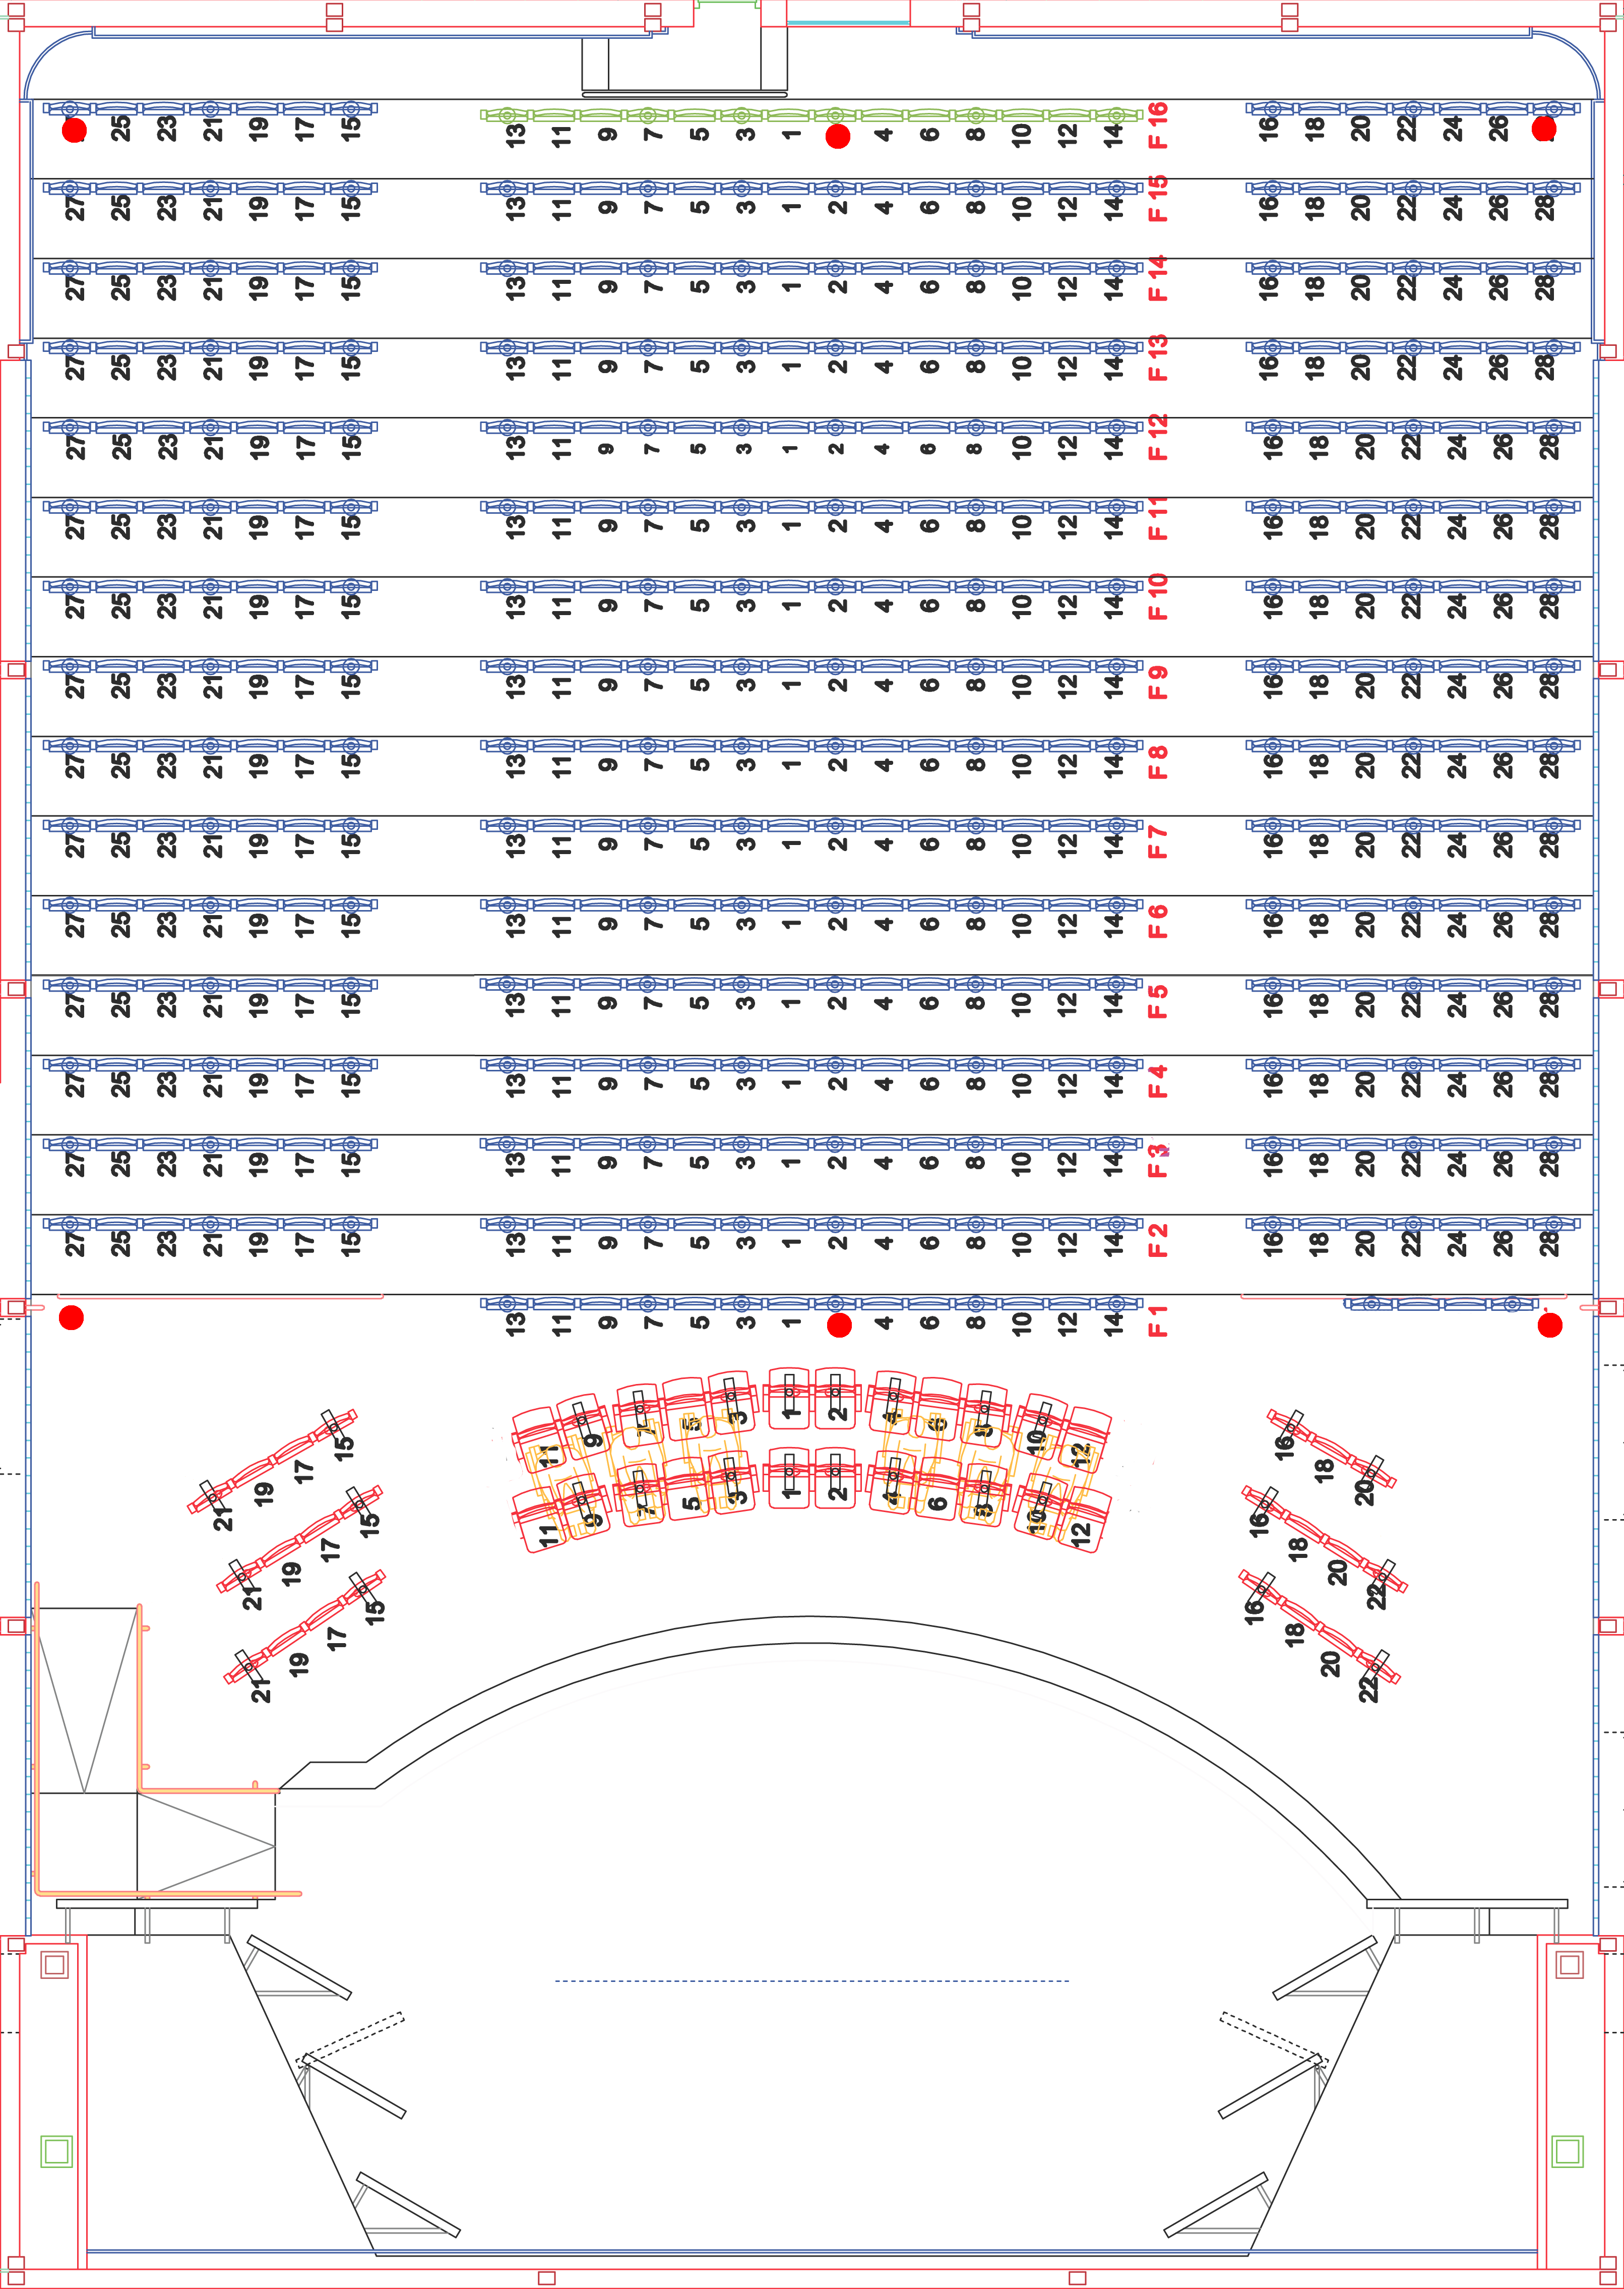
\includegraphics[scale=0.1]{../imagenes/auditorio_butacas_prueba.png}
			        \centering
			        \caption{Posiciones de las grabaciones utilizadas para el test de prueba.}
			        \label{fig:posicionesTestPrueba}
                \end{figure}
                    
                    \item \textbf{¿Cuál es tipo de análisis de datos?}: Para el análisis de los datos, se ha optado por realizar un análisis del coeficiente $\alpha$ de acuerdo con las especificaciones de la norma ISO-10399 \cite{ISO10399}. En dicha norma, se proporciona una tabla que muestra el número de respuestas correctas necesarias para concluir que dos eventos son diferentes con una determinada incertidumbre para un determinado número de respuestas totales.
                \end{itemize}
 
            \subsection{Procedimiento del test previo}
                Una vez determinadas todas las características del test previo, se empieza a realizar el test de forma individual a cada uno de los diez participantes. La sala donde se realizaron las escuchas fue una de las salas de laboratorio del Centro de Investigación en Tecnologías Software y Sistemas Multimedia para la Sostenibilidad (CITSEM). Esta sala se encuentra aislada de las zonas de tránsito y sus ventanas no dan a zonas con tráfico. De esta forma, se pueden controlar fácilmente las fuentes de ruido ajenas al experimento. Es importante remarcar que, debido a la pandemia producidad por la COVID-19, las ventanas tenían que estar abiertas en todo momento con el fin de conseguir unas condiciones de ventilación apropiadas que evitaran posibles contagios. Este es el motivo por el que se optara por una sala cuyas ventanas no dieran a fuentes de ruido externas.
                
                El equipo utilizado consistió en un ordenador portátil con sistema operativo Debian con 12GB de memoria RAM y unos auriculares Tascam-TH02. La escucha de los diferentes audios y la inclusión de las respuestas se realiza mediante una interfaz gráfica diseñada en el lenguaje de programación Python utilizando la librería de código abierto GTK, como ya se explicó en el apartado ``Desarrollo de aplicación en Python''. En la figura \ref{fig:interfazInicial} se puede observar la interfaz utilizada en el test previo. Previa a las escuchas por parte de los participantes, se aseguró de que las señales se reprodujeran con un nivel adecuado. Al principio del test, se les explicaba a los participantes las carácterísticas del test que iban a relizar, así como el número de preguntas y en qué propiedades debían fijarse para facilitarles su realización. También se les pedía que leyeran y firmara un ``consentimiento informado'' cuya estructura puede consultarse en el anexo X. Una vez finalizada la realización del test y ,debido al carácter no definitivo del mismo, se les preguntó sobre posibles mejoras que se podían hacer para facilitar su realización como cambios en la interfaz gráfica, la inclusión de audios de ejemplo, etc.
                
                 \begin{figure}[H]
                    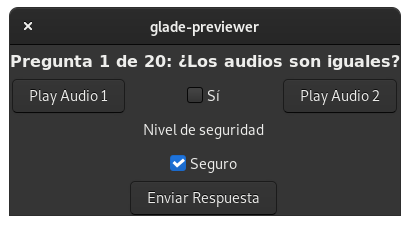
\includegraphics[scale=0.6]{../imagenes/uiIni.png}
			        \centering
			        \caption{Interfaz gráfica para la realización del test previo.}
			        \label{fig:interfazInicial}
                \end{figure}
                
        \section{Experimentos finales}
            En este apartado se analizan las características y procedimientos utilizado en los experimentos finales.     
            
            \subsection{Características de los test finales}
                Como ya se comentó en el análisis del estado del arte, no existe un consenso sobre la mejor forma de realizar un test subjetivo de audio. Algunos estudios como \cite{Tejada2020}, \cite{delaPrida2019} y \cite{delaPrida2021} hacen sugerencias sobre qué características pueden funcionar mejor en función de lo que se pretenda analizar en dicho test. Para nuestro caso particular, se ha vuelto a optar por seguir las recomendaciones propuestas en \cite{Tejada2020} respondiendo a las preguntas que en él se plantean. Como ya se comentó en el apartado de ``Toma de datos'', se tuvieron que repetir los test de audio debido a un fallo en el procesado de las grabaciones. A pesar de esto, las características de ambas pruebas son prácticamente idénticas. Por este motivo, se engloban todas ellas en el mismo apartado. Dentro de cada subapartado se comentan, si existen, las diferencias que pueda haber entre ambos.
            
                \begin{itemize}
                
                    \item \textbf{¿En qué categoría se engloba el estudo?}: Al igual que en el test previo, se pretende determinar la sensibilidad que tienen las personas para distinguir las diferencias perceptuales al escuchar sonidos cuando se encuentran en distintas posiciones respecto de la fuente acústica. Por este motivo, se puede concluir que este test se encuentra englobado dentro de los que se consideran como de Sensibilidad.
                    \item \textbf{¿Qué tipo de test es el más adecuado?}: Para el estudio que se pretende hacer, existen numerosos tipos de test que pueden arrojar datos interesantes. Entre ellos, los dos más habituales son los de referencia oculta como ABX o los Duo-Trio. No obstante, se ha optado por repetir el tipo de test utilizado en el estudio previo; es decir 2-AFC o \textit{Same-Different}. Los motivos que han llevado a esta elección han sido la facilidad de implementación y codificación, su simpleza que lo hace apropiado para todo tipo de participantes y que permite arrojar resultados bastante fiables mediante un análisis relativamente sencillo usando modelos Thurstonianos, además de que existen normas internacionales que permiten obtener resultados extra que pueden ser interesantes de comparar con los de dichos modelos.
                    \item \textbf{¿Participantes expertos o inexpertos?, ¿cuántos necesito?}: A la hora de plantear el experimento, desde un primer momento se planteó como una situación que afectaba a la población general. Por este motivo, se consideró que no era relevante que los participantes tuvieran una experiencia particular en la realización de este tipo de test, aunque obviamente, es necesario que no padezcan de ningun problema auditivo que afecte a su nivel de audición, ya sea por la edad, enfermedad, etc. A pesar de todo esto, se consideró que todas personas participantes debían pasar por una breve sesión de entrenamiento previo para que supieran de antemano en qué elementos de los sonidos tenían que fijarse. Estas indicaciones vienen reflejadas en las normas \cite{UIT1116, UIT1534, UIT1284, EBU3286, UIT1285, UIT1286} que muestran la utilidad de este tipo de entrenamientos para obtener mejores resultados.
                
                    En cuanto al número de participantes totales, se siguieron las recomendaciones de las mismas normas, así como las conclusiones extraídas de \cite{Tejada2020} y de los otros experimentos consultados de temática similar \cite{2005IWitew, 2019DJSchlit, 2016SKlockgether, 2019LKritly, 2019GPulvirenti, 2019MNowak, 2011VEmiya}. De esta forma, se concluyó que el número de participantes debían de ser de un mínimo de 30 personas.
                    \item \textbf{¿Qué tipo de señal utilizo?}: Las señales utilizadas para la realización del primer test fueron los archivos de audio generados tras la convolución de la voz femenina obtenida en la web de ``OpenAir'', perteneciente a la universidad de York, con cada una de las respuestas impulsivas grabadas en el salón de actos de la ETSIST de la UPM. El proceso de obtención de dichas respuestas se encuentra explicado en el apartado de ``Toma de datos''. Se trata de un total de 100 archivos de audio de 7 segundos de duración. Esta duración se encuentra dentro de los límites marcados por \cite{UIT1116, UIT1534, UIT1284, EBU3286, UIT1285, UIT1286} para evitar que los oyentes se ``acostumbren'' al  sonido. Así mismo, se encuentra dentro del abánico de duraciones que se ha observado en distintos proyectos de similares características. \newline
                
                    Para el segundo test, se optó por utilizar diréctamente las respuestas al impulso obtenidas tras el procesado que realiza el software \textit{Dirac}, como ya se explica también en el apartado de ``Toma de datos''. En este caso, se utilizan un total de 83 archivos distintos de 2 segundos de duración. Al igual que en la prueba anterior, la duración se encuentra dentro de los límites marcados por \cite{UIT1116, UIT1534, UIT1284, EBU3286, UIT1285, UIT1286}, así como otros estudios para evitar la fatiga auditiva y que los participantes se acostumbren a los estímulos.
                
                    Para la realización de ambos experimentos, el volumen al cual se reproducen las señales no es relevante, siempre y cuando no se modifique a lo largo de toda la sesión; por lo que el participante puede escoger el que le sea más cómodo, con la única restricción de que el volumen debe ser el mismo para la escucha de los dos audios que conforman cada pregunta.
                    \item \textbf{¿Cuál es el tipo de análisis de datos?}: para los test finales se han optado por dos análisis diferentes. Por un lado, se mantiene el análisis del coeficiente $\alpha$ siguiendo las especificicaciones de la norma ISO-10399\cite{ISO10399} y las tablas que ofrece en sus anexos. Por otro lado, se realiza un análisis mediante la utilización de modelos thursthonianos. Estos modelos permiten obtener un coeficiente llamado $d'$ el cual aporta información cuantitativa sobre una determinada información subjetiva (en este caso, lo diferentes que son un grupo de parejas de audios). En el capítulo de ``Estado del arte'' se dispone de información más concreta sobre estos modelos. Ambos análisis, el de norma ISO-10399 y los modelos thursthonianos se realizan para dos diferentes disposiciones de los datos: según la distancia del punto medio de la posición de los dos audios respecto de la fuente, y según la distancia a la que se encuentre la posición de ambos audios.
                     
                \end{itemize}
            \subsection{Procedimiento del test final}
        
                \subsubsection*{Localización}
                    En primer lugar, se organizaron los turnos para la realización del test. El espacio escogido para la realización de las escuchas consistió en un laboratorio del CITSEM localizado en el Campus Sur de la UPM. Se escogió esta localización porque, debido a la situación pandémica producida por el COVID-19, era necesario que las ventanas estuvieran abiertas en todo momento. Se planteó la utilización de aparatos de depuración del aire, pero su ruido era comparable o más molesto todavía que la realización del mismo con las ventanas abiertas. No obstante, se escogió una localización donde las ventanas daban a una zona poco transitada, tanto por peatones como por vehículos, de forma que se conseguía un ambiente suficientemente controlado y silencioso. Si antes de comenzar el test se consideraba que el ruido externo era mayor del habitual, se cerraban las ventanas durante su realización y se volvían a abrir al finalizar el experimento.
            
                \subsubsection*{Material utilizado}
                    Para la realización de ambos test se utilizó el mismo material que en el test preliminar. En concreto:
                    \begin{itemize}
                        \item Ordenador portátil con S.O. Debian 11 con procesador \textit{intel} i5 y 12GB de RAM.
                        \item Auriculares Tascam-TH02.
                        \item declaraciones de consentimiento.
                        \item software \textit{Gnome Builder} para la ejecución de la aplicación.
                    \end{itemize}
                
                \subsubsection*{Realización del test}
                    En primer lugar, todas las personas participantes debían inscribirse en las franjas habilitadas en un calendario con el fin de poder organizar las entradas y salidas evitando que se produjeran acumulaciones de personas en espacios cerrados. Una vez inscritas y cuando llegaba su turno, se les explicaba brevemente en qué consistía el experimento del que iban a formar parte y se les daba a leer una hoja de información al participante en el que se explica en mayor detalle las particularidades del test, las partes de la que consta, así como información relevante en temas de salud y protección de datos. Una vez leído, debían rellenar una declaración responsable aceptando los aspectos marcados en el documento anterior. Los modelos de ambos documentos pueden consultarse en su totalidad en el Anexo X.
                
                    A continuación daba comienzo el test con el tutorial. En él se le presentan al participante tres de las posibilidades que podría encontrarse (que los audios fueran de la misma posición, que fueran de filas distintas y que fueran de butacas distintas de la misma fila). Como el objetivo de este tutorial es que sepan identificar qué aspectos determinan que dos audios sean iguales o diferentes, para los tres casos se optó por utilizar casos críticos, estos son aquellos que se utilizaban las mismas posiciones que en el test previo, donde las posiciones estaban lo más separadas posibles (ver figura X). La reproducción de los audios se podía repetir el número de veces que se considerara necesario. En la figura \ref{fig:interfazTutorial} puede observarse la interfaz de dicha parte.
                
                    \begin{figure}[H]
                        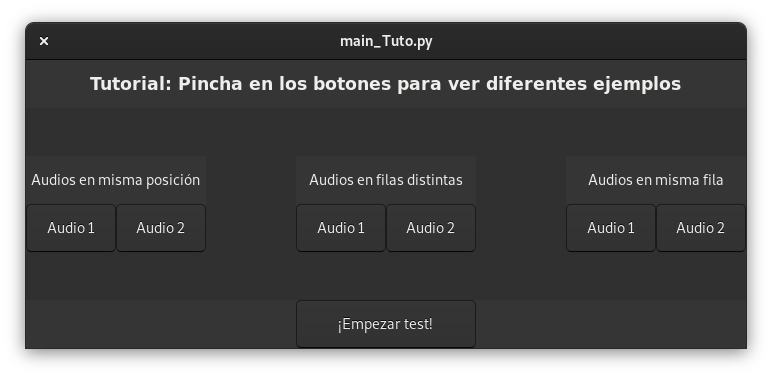
\includegraphics[scale=0.6]{../imagenes/interfaz_tutorial.png}
			            \centering
			            \caption{Aapriencia del entrenamiento previo}
			            \label{fig:interfazTutorial}
                    \end{figure}
                
                    Una vez el participante consideraba que estaba preparado, pulsaba el botón de ``Comenzar el test'' para dar inicio a la segunda parte.
                
                    En esta segunda parte al usuario se le presentan dos audios convolucionados de forma aleatoria y debe determinar si lo que percibe son dos audios que suenan igual o no. Por otro lado, el participante debe especificar si se encuentra seguro de su respuesta. El usuario puede repetir la reproducción de los audios las veces que quiera, pero debe esperar a que el audio termine de reproducirse antes de poder escoger si repetirlo o escuchar el otro audio. No existe la opción de ``No sabe/no contesta'', por lo que en caso de no poder decidirse, el usuario debe escoger una de las dos opciones de forma aleatoria y marcar la opción de ``no seguro''. Una vez ha decidido su respuesta, debe pinchar en el botón de ``Enviar respuesta'' para que se le presenten los dos siguientes audios. Esto permite que, en caso de duda, los participantes puedan modificar su respuesta hasta que pulsen dicho botón. A partir de ahí, no se permite volver atrás o modificar las respuestas. El experimento termina tras las 25 rondas de preguntas. Una vez terminada esta parte, el trabajo de las personas voluntarias ha terminado y pueden marcharse para dar comienzo el de la siguiente persona. En la figura \ref{fig:interfazTestFin} puede observarse la interfaz utilizada para la realización de esta segunda parte.
                
                    \begin{figure}[H]
                        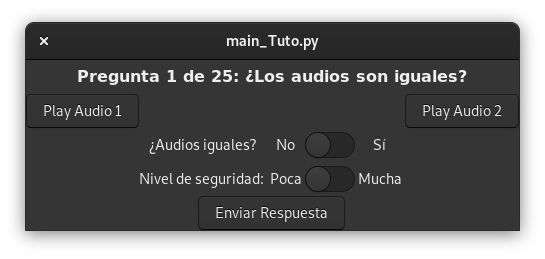
\includegraphics[scale=0.6]{../imagenes/interFin.png}
			            \centering
			            \caption{Apariencia de la interfaz del test.}
			            \label{fig:interfazTestFin}
                    \end{figure}
                
                    Todos los resultados se almacenan durante la ejecución del experimento en un archivo con terminación ``.csv'', que es el que se utiliza posteriormente para el análisis de los datos.
                
                    Para la realización del test participaron un total de 31 personas para la primera versión de este test y 34 personas en la segunda. Las edades del primer test estaban comprendidas entre los 18 y los 60 años, mientras que la segunda las edades se comprendieron en el rango de los 18 a los 33 años. En la figura \ref{fig:participantes} se puede observar una imagen de varios de los partcipantes durante el transcurso del test.
                
                    \begin{figure}
                        \includegraphics[scale=0.45]{../imagenes/participantes.png}
			            \centering
			            \caption{Varios de los participantes durante el transcurso de los test.}
			            \label{fig:participantes}
                    \end{figure}
    
    \chapter{Resultados de los experimentos}
    En este apartado se muestran los resultados obtenidos de los diferentes test perceptuales que se han realizado a lo largo del proyecto. 
    \section{Resultados del test previo}
        Como ya se comentó en apartados anteriores, en este test previo el objetivo consiste en comprobar que los participantes podían realmente distinguir los estímulos cuando se correspondían a las de las posiciones más alejadas entre sí. Del mismo modo, se han agrupado los resultados en función de cuatro casos posibles: Butacas separadas horizontalmente, butacas separadas verticalmente, butacas separadas tanto vertical como horizontalmente y butacas en la misma posición. Este test, como ya se comentó anteriormente, fue realizado por un total de 10 personas, obteniéndose un total de 70 respuestas. Los resultados totales pueden observarse en la tabla \ref{tablaTestPrevio}, mientras que la tabla con cada uno de los resultados individuales con el nombre de cada posición exacta se encuentra en el anexo X.
        
        \begin{table}[H]
			\begin{center}
			\begin{scriptsize}
			\begin{tabular}{| c | c | c | c | c | c |}
			    \hline
				\textbf{Separación butacas}&\textbf{Respuestas}&\textbf{Total iguales}&\textbf{Total diferentes}&\textbf{Duda iguales}&\textbf{Duda diferentes}\\ \hline
                Horizontal&27&9&18&2&2\\ \hline
                Vertical&10&1&9&0&1\\ \hline
                Horizontal y vertical&23&5&18&1&2\\ \hline
                Misma posición&10&9&1&1&0\\ \hline
			\end{tabular}
			\caption{Resultados del test previo.}
			\label{tablaTestPrevio}
			\end{scriptsize}
			\end{center}	
		\end{table}	
	\section{Resultados del test final}
	    Para este test, se han agrupado los resultados de dos formas de manera que resulta más fácil entenderlos para el análisis que se realiza más adelante en el apartado de ``Análisis estadístico''. La primera forma de organización es en función de la distancia relativa entre butacas. Esta separación se expresa en la primera columna con intervalos de la forma $[x-y)$ donde se expresa el rango de distancias en las que se incluyen las respuestas. Un ejemplo es el intervalo $[2-3)$ incluye todas las respuestas en el que la distancia relativa entre butacas se encuentra entre los 2 metros (incluidos) y los 3 metros (sin incluir). Para este tipo de agrupación, los resultados son los mostrados en la tabla \ref{tablaTestButacas} que muestran los resultados de las 34 personas que participaron en el test produciendo un total de 850 respuestas.
	    
	    \begin{table}[H]
			\begin{center}
			\begin{scriptsize}
			\begin{tabular}{| c | c | c | c | c | c |}
			    \hline
				\textbf{Distancia [m]}&\textbf{Respuestas}&\textbf{Iguales}&\textbf{Diferentes}&\textbf{Duda iguales}&\textbf{Duda diferentes}\\ \hline
                (0-2)&61&40&21&11&9\\ \hline
                [2-3)&76&40&36&11&16\\ \hline
                [3-4)&102&47&55&14&14\\ \hline
                [4-5)&111&30&81&13&29\\ \hline
                [5-6)&95&24&71&9&21\\ \hline
                [6-7)&78&11&67&6&10\\ \hline
                [7-8)&70&9&61&2&4\\ \hline
                [8-9)&52&4&48&3&9\\ \hline
                [9-10)&62&3&59&1&8\\ \hline
                [10-11)&47&1&46&0&3\\ \hline
                [11-12)&33&1&32&0&2\\ \hline
                [12-14)&33&1&32&1&0\\ \hline
                [14-18)&24&0&24&0&1\\ \hline
			\end{tabular}
			\caption{Resultados del test final en función de la distancia relativa entre butacas.}
			\label{tablaTestButacas}
			\end{scriptsize}
			\end{center}	
		\end{table}
		
		La otra forma de organización de los datos es ordenando los datos en función de la distancia relativa a la fuente sonora (considerando esta como un origen de coordenadas). En este caso, la agrupación sigue la misma nomenclatura que en el caso anterior, sólo que esta vez el intervalo $[x-y)$ se corresponde con las distancias a la fuente, en vez de la posición relativa entre butacas. Haciendo esta organización, los datos se reparten de la forma que se muestra en la tabla \ref{tablaTestFuente}
		
		\begin{table}[H]
			\begin{center}
			\begin{scriptsize}
			\begin{tabular}{| c | c | c | c | c | c |}
			    \hline
				\textbf{Distancia [m]}&\textbf{Respuestas}&\textbf{Iguales}&\textbf{Diferentes}&\textbf{Duda iguales}&\textbf{Duda diferentes}\\ \hline
                [6-8)&15&5&10&2&2\\ \hline
                [8-10)&35&10&25&2&3\\ \hline
                [10-11)&32&8&24&2&7\\ \hline
                [11-12)&54&13&41&7&7\\ \hline
                [12-13)&56&15&41&4&5\\ \hline
                [13-14)&67&14&53&6&9\\ \hline
                [14-15)&102&23&79&10&10\\ \hline
                [15-16)&100&19&81&4&12\\ \hline
                [16-17)&84&18&66&4&12\\ \hline
                [17-18)&63&10&53&3&11\\ \hline
                [18-19)&95&21&74&3&15\\ \hline
                [19-20)&62&19&43&11&9\\ \hline
                [20-21)&44&19&25&9&10\\ \hline
                [21-24]&41&23&18&6&4\\ \hline
			\end{tabular}
			\caption{Resultados del test final en función de la distancia relativa a la fuente.}
			\label{tablaTestFuente}
			\end{scriptsize}
			\end{center}	
		\end{table}
		
		Para el cálculo de ambas distancias, se ha generado un script en Python que extrae la información de la posición de recepción de cada fichero de audio que se encuentra en el nombre de dicho archivo y las distancias medidas presencialmente en el auditorio (toda esta información se comentó en el apartado de ``Toma de datos'').
		
		Tomando esta información se hace el cálculo de las distancias para todos los casos que se han producido durante la realización de los test y que han quedado recogidas en el fichero csv. En la figura X se puede observar un ejemplo gráfico sobre cómo se han calculado dichas distancias y en el anexo X se puede consultar el código de Python en su totalidad.
    
    \chapter{Análisis estadístico}    
    
    En este apartado, se muestran los diferentes análisis que se han realizado para los diferentes test; así como los procedimientos utilizados para su obtención.
        
    \section{Análisis del test previo}
        Para este test sólo se pretende comprobar si las personas eran capaces de distinguir entre audios en posiciones muy diferentes. Por este motivo, se decidió realizar un análisis más sencillo que en el caso del test final. Más concretamente, se optó por utilizar la tabla A1 del anexo A de la norma UNE-EN ISO 10399, así como la ecuación \ref{eq:alpha} ya mostrada en el capítulo de ``Estado del arte''.
            
        Aplicando dichos recursos se obtienen las tablas \ref{tablaResultadosDuda} y \ref{tablaResultadosSinDuda} en la que se incluyen todas las respuestas y únicamente las que se marcaron como ``seguras'' por parte de los participantes respectivamente:
            
        \begin{table}[H]
	    \begin{center}
		\begin{scriptsize}
		\begin{tabular}{| c | c | c | c || c |}
			\hline
			\textbf{Separación butacas}&\textbf{Respuestas}&\textbf{Iguales}&\textbf{Diferentes}&\textbf{$\alpha$-risk}\\ \hline
            Horizontal&27&9&18&0.1\\ \hline
            Vertical&10&1&9&0.01\\ \hline
            Horizontal y vertical&23
            &5&18&0.01\\ \hline
            Misma posición&10&9&1&NO\\ \hline
		\end{tabular}
		\caption{Resultados del test previo.}
		\label{tablaResultadosDuda}
		\end{scriptsize}
		\end{center}	
		\end{table}	
		
		\begin{table}[H]
			\begin{center}
			\begin{scriptsize}
			\begin{tabular}{| c | c | c | c || c |}
			    \hline
				\textbf{Separación butacas}&\textbf{Respuestas}&\textbf{Iguales}&\textbf{Diferentes}&\textbf{$\alpha$-risk}\\ \hline
                Horizontal&23&7&16&0.05\\ \hline
                Vertical&9&1&8&0.05\\ \hline
                Horizontal y vertical&20&4&16&0.01\\ \hline
                Misma posición&9&8&1&NO\\ \hline
			\end{tabular}
			\caption{Resultados del test previo considerando las respuestas marcadas como ``Sin duda''.}
			\label{tablaResultadosSinDuda}
			\end{scriptsize}
			\end{center}	
		\end{table}
		
		Como se puede observar de las tablas ya mencionadas, existen diferencias estadísticamente significativas cuando se separan los puntos de escucha. Dicho efecto se sigue manteniendo cuando se suprimen las respuestas marcadas como ``No seguras''. Por este motivo, se considera probada nuestra primera hipótesis y se decidió continuar con el estudio.
		
		Los valores concretos obtenidos para $\alpha$-risk no son realmente importantes, puesto que el número de datos es relativamente pequeño y la repetición de dicho experimentos podría producir que dichos valores fluctuaran. Para este caso, el experimento resulta válido al obtener valores inferiores y/o iguales a 0.1, que es lo que se ha obtenido (excepto para las respuestas en la misma posición donde se esperaba que no pudiera obtener un valor para $\alpha$-risk).
		
		También se obtienen los resultados esperados para los casos en que ambos audios se encuentran en la misma posición, donde la amplia mayoría de las personas participantes no percibían los estímulos como diferentes.
		
    \section{Análisis del test final}
        Para el análisis del test final, se realizan dos análisis de datos diferentes para cada una de las dos formas de agrupación de los datos (distancia relativa a la fuente y distancia relativa entre las dos posiciones de butacas). El primer análisis se hará mediante el seguimiento de la norma UNE-EN ISO 10399 que ya se utilizó en el test previo, mediante la tabla A.1 de la norma y la ecuación \ref{eq:alpha}.
        
        Por otro lado, se realiza un análisis mediante modelos thursthonianos. Para ello, se genera un script en el lenguaje de programación estadística ``R'' para utilizar el paquete ``SensR''\footnote{https://cran.r-project.org/web/packages/sensR/index.html}. Este paquete permite obtener de forma sencilla los valores del coeficiente $d'$, así como su desviación estandar. En el anexo X puede consultarse el script.
        
        
		\subsection{Distancia relativa a la fuente}
		    Aplicando el mismo procedimiento explicado en apartado de ``Conceptos teóricos'', se obtienen los resultados para el análisis mediante la norma UNE-EN ISO 10399 para todas las respuestas y sólo para las marcadas como ``sin duda'', respectivamente. También se utiliza el lenguaje de programación R y el paquete antes mencionado y así obtener el coeficiente $d'$ y su desviación estándar ($\sigma$). Todos los valores de ambos análisis están representados en las tablas \ref{tablaFuenteDuda} y \ref{tablaFuenteSinDuda}. Para la parte del análisis mediante modelos thursthonianos se generan además las figuras \ref{fig:ThurstFuenteDuda} y \ref{fig:ThurstFuenteSinDuda} que muestran de forma gráfica la variación de dicho coeficiente. El procedimiento para obtener el análisis con ``R'' es el siguiente: en primer lugar se introduce el núemero total de respuestas, así como el número de respuestas ``correctas'' (entendiéndose como correctas aquellas respuestas en las que los participantes hayan identificado los estímulos como diferentes). A continuación, hay que indicar a la función qué tipo de test se ha realizado para que el cálculo de los coeficientes sea el correcto. En nuestro caso, el test se corresponde con un ``\textit{2-AFC}'', ya quel participante estaba forzado a seleccionar una de las dos opciones sin posibilidad de escoger una opción intermedia.
		    
		    \begin{table}[H]
			\begin{center}
			\begin{scriptsize}
			\begin{tabular}{| c | c | c | c || c | c | c |}
			    \hline
				\textbf{Distancia [m]}&\textbf{Resultados}&\textbf{Total iguales}&\textbf{Total diferentes}&\textbf{$\alpha$-Risk}&\textbf{$d'$}&\textbf{$\sigma (d')$}\\ \hline
                [6-8)&15&5&10&0.2&0.609&0.473\\ \hline
                [8-10)&35&10&25&0.05&0.800&0.318\\ \hline
                [10-11)&32&8&24&0.01&0.954&0.341\\ \hline
                [11-12)&54&13&41&0.001&0.995&0.264\\ \hline
                [12-13)&56&15&41&0.001&0.876&0.254\\ \hline
                [13-14)&67&14&53&0.001&1.146&0.244\\ \hline
                [14-15)&102&23&79&0.001&1.066&0.195\\ \hline
                [15-16)&100&19&81&0.001&1.242&0.204\\ \hline
                [16-17)&84&18&66&0.001&1.120&0.217\\ \hline
                [17-18)&63&10&53&0.001&1.414&0.269\\ \hline
                [18-19)&95&21&74&0.001&1.087&0.203\\ \hline
                [19-20)&62&19&43&0.01&0.715&0.236\\ \hline
                [20-21)&44&19&25&NO&0.243&0.269\\ \hline
                [21-24]&41&23&18&NO&0.000&NA\\ \hline
			\end{tabular}
			\caption{Valores de $\alpha$-risk, $d'$ y su desviación estandar para los resultados totales agrupados en función de la distancia a la fuente según la norma UNE-EN ISO 10399 y aplicando modelos thursthonianos, respectivamente.}
			\label{tablaFuenteDuda}
			\end{scriptsize}
			\end{center}	
		    \end{table}
		    
		    \begin{table}[H]
			\begin{center}
			\begin{scriptsize}
			\begin{tabular}{| c | c | c | c || c | c | c |}
			    \hline
				\textbf{Distancia [m]}&\textbf{Respuestas}&\textbf{Total iguales}&\textbf{Total diferentes}&\textbf{$\alpha$-risk}&\textbf{$d'$}&\textbf{$\sigma (d')$}\\ \hline
                [6-8)&11&3&8&0.2&0.855&0.571\\ \hline
                [8-10)&30&8&22&0.01&0.881&0.347\\ \hline
                [10-11)&23&6&17&0.05&0.906&0.399\\ \hline
                [11-12)&40&6&34&0.001&1.466&0.342\\ \hline
                [12-13)&47&11&36&0.001&1.026&0.285\\ \hline
                [13-14)&52&8&44&0.001&1.443&0.298\\ \hline
                [14-15)&82&13&69&0.001&1.415&0.236\\ \hline
                [15-16)&84&15&69&0.001&1.302&0.226\\ \hline
                [16-17)&68&12&56&0.001&1.314&0.252\\ \hline
                [17-18)&49&7&42&0.001&1.510&0.313\\ \hline
                [18-19)&77&18&59&0.001&1.027&0.223\\ \hline
                [19-20)&42&8&34&0.001&1.239&0.315\\ \hline
                [20-21)&25&10&15&No&0.358&0.359\\ \hline
                [21-24]&31&17&14&No&0&NA\\ \hline
			\end{tabular}
			\caption{Valores de $\alpha$-risk, $d'$ y su desviación estandar  para los resultados marcados como ``Sin duda'' agrupados en función de la distancia a la fuente según la norma UNE-EN ISO 10399 y aplicando modelos thursthonianos, respectivamente.}
			\label{tablaFuenteSinDuda}
			\end{scriptsize}
			\end{center}	
		    \end{table}
		    
		    
		    
		    \begin{figure}[H]
                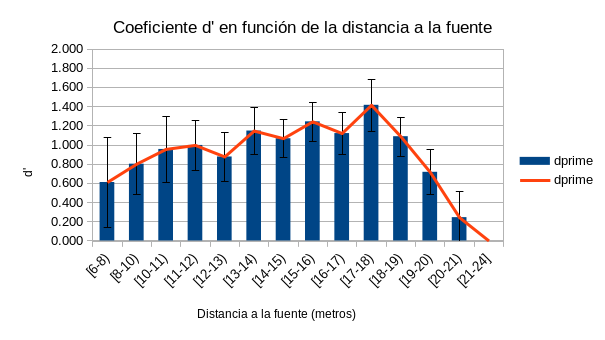
\includegraphics[scale=0.7]{../imagenes/analisisThurstFuenteDuda.png}
			    \centering
			    \caption{Coeficientes $d'$ en función de la distancia a la fuente.} 
			    \label{fig:ThurstFuenteDuda}
            \end{figure}
            
            \begin{figure}[H]
                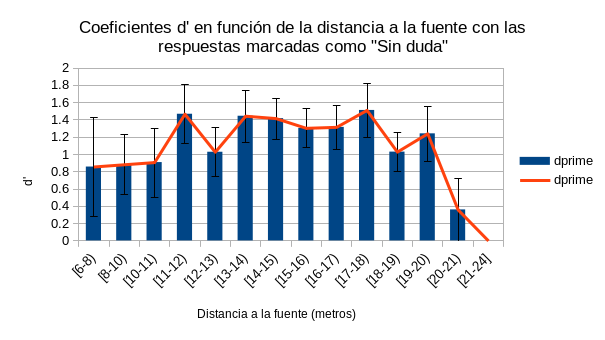
\includegraphics[scale=0.7]{../imagenes/analisisThurstFuenteSinDuda.png}
			    \centering
			    \caption{Coeficientes $d'$ en función de la distancia a la fuente cuando las respuestas están marcadas como ``Sin duda''.} 
			    \label{fig:ThurstFuenteSinDuda}
            \end{figure}

            Como se puede observar en las tablas y figuras antes mencionadas, el comportamiento para ambos procedimientos es bastante similar. Hay que tener en cuenta que para $\alpha$-risk, cuanto más pequeño es el valor, más estadísticamente representativa es la diferencia, mientras que para los modelos thursthonianos, se produce a la inversa; cuanto más grande es el valor de $d'$, más diferentes son los estímulos.
            
            En ambos casos, se observa que las diferencias aumentan conforme aumenta la distancia respecto de la fuente, pero llegada una determinada distancia, las diferencias comienzan a dejar de ser perceptibles hasta llegar a posiciones donde las posibles diferencias pueden considerarse debidas al azar.
            
            La mayor diferencia entre ambos sistemas se encuentra en lo que podríamos denominar como ``sensibilidad''. La norma UNE-EN ISO 10399 es menos sensible a las variaciones puntuales del número de respuestas consideradas correctas; además de que los cambios que se producen son mucho más abruptos ya que sólo existen cinco posibles valores para $\alpha$-risk (0.2, 0.05, 0.01, 0.001 y que no pueda obtenerse el valor).
            
            Los modelos thursthonianos, por otra parte, son mucho más sensibles, ya que ligeras variaciones en los resultados, producen variaciones en los valores de $d'$. Al mismo tiempo, se dispone de todo un rango contínuo de valores que dicho coeficiente puede obtener. Esto permite que las representaciones gráficas de las variaciones de $d'$ muestren mejor el comportamiento psicoacústico de los estímulos y analizar si existe una tendencia que estas pueden seguir, como es el caso de nuestro experimento.
            
            Un ejemplo de esto puede observarse en los casos de la tabla \ref{tablaFuenteDuda}. En esta tabla, se ve como para el caso del análisis mediante la norma, el descenso se produce a partir de la distancia de [19-20) metros, mientras que en los modelos thursthonianos, el decaimiento se produce antes, a partir de la distancia [18-19) metros. Lo mismo ocurre con el caso de la tabla \ref{tablaFuenteSinDuda}, donde los decaimientos vuelven a producirse en las mismas distancias. Para tener una idea de este comportamiento sobre el espacio del auditorio, se presenta la figura \ref{fig:dprimeauditorio}, donde se representa el comportamiento de $d'$ (la percepción de diferencia entre parejas de estímulos) en función de dicha distancia en la fuente, pero representado sobre el plano del auditorio directamente mediante un diagrama de colores en el que las zonas verdes representan valores bajos de dichas diferencias perceptuales y las zonas rojas representan valores elevados. Las zonas sin pintar corresponden a zonas donde o bien no se han tomado medidas, o bien el valor de las diferencias perceptuales ($d'$) es nulo.
            
            \begin{figure}[H]
                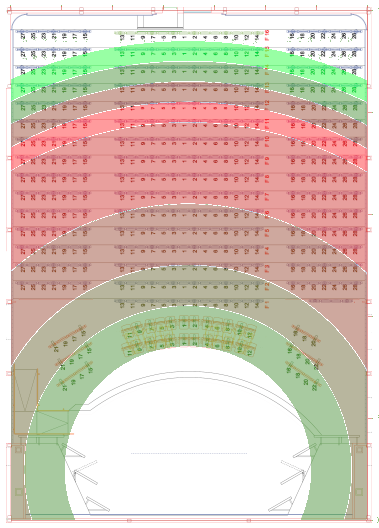
\includegraphics[scale=0.9]{../imagenes/auditoriodprime.png}
			    \centering
			    \caption{Coeficientes $d'$ en función de la distancia a la fuente representado sobre el plano del auditorio. Los valores verdes representan un valor bajo de $d'$; mientras que los rojos representan valores elevados.} 
			    \label{fig:dprimeauditorio}
            \end{figure}
        
        \subsection{Distancia relativa entre butacas}
            Para este apartado se vuelven a aplicar tanto los procedimientos de la norma UNE-EN ISO 10399, como los modelos thusthonianos. De ambos análisis se obtienen las tablas \ref{tablaButacasDuda} y \ref{tablaButacasSinDuda}, así como las figuras \ref{fig:ThurstButacasDuda} y \ref{fig:ThurstButacasSinDuda}. De nuevo, para los modelos thursthonianos, se ha determinado que el protocolo es ``\textit{2-AFC}'' para que la función de R pueda realizar de forma correcta la estimación del valor $d'$.
            
            Como se puede observar en las tablas recien mencionadas, los participantes empiezan a notar diferencias a partir de que la distancia entre butacas se encuentra a partir de los [3-4) metros, aunque este efecto se retrasa hasta los [4-5) metros si suprimimos las respuestas marcadas como ``Con duda''. Una vez ahí, las diferencias se mantienen estadísticamente representativas con el máximo nivel de seguridad que ofrece la norma, ya que la probabilidad de que los eventos sean iguales cuando, en realidad, se han percibido como diferentes, es de 0.001. En los resultados obtenidos no hay un momento en el que dicha probabilidad decrezca.
            
            \begin{table}[H]
			\begin{center}
			\begin{scriptsize}
			\begin{tabular}{| c | c | c | c || c | c | c |}
			    \hline
				\textbf{Distancia [m]}&\textbf{Respuestas}&\textbf{Total iguales}&\textbf{Total diferentes}&\textbf{$\alpha$-risk}&\textbf{$d'$}&\textbf{$\sigma (d')$}\\ \hline
                (0-2)&61&40&21&NO&0.000&NA\\ \hline
                [2-3)&76&40&36&NO&0.000&NA\\ \hline
                [3-4)&102&47&55&0.05&0.139&0.176\\ \hline
                [4-5)&111&30&81&0.001&0.865&0.18\\ \hline0
                [5-6)&95&24&71&0.001&0.942&0.197\\ \hline
                [6-7)&78&11&67&0.001&1.521&0.249\\ \hline
                [7-8)&70&9&61&0.001&1.603&0.270\\ \hline
                [8-9)&52&4&48&0.001&2.017&0.362\\ \hline
                [9-10)&62&3&59&0.001&2.349&0.384\\ \hline
                [10-11)&47&1&46&0.001&2.868&0.583\\ \hline
                [11-12)&33&1&32&0.001&2.654&0.615\\ \hline
                [12-14)&33&1&32&0.001&2.654&0.615\\ \hline
                [14-18)&24&0&24&0.001&$\infty$&NA\\ \hline
			\end{tabular}
			\caption{Valores de $\alpha$-risk, $d'$ y su desviación estándar para los resultados totales agrupados en función de la distancia entre butacas según la norma UNE-EN ISO 10399 y aplicando modelos thursthonianos, respectivamente.}
			\label{tablaButacasDuda}
			\end{scriptsize}
			\end{center}	
		    \end{table}
		    
		    \begin{table}[H]
			\begin{center}
			\begin{scriptsize}
			\begin{tabular}{| c | c | c | c || c | c | c |}
			    \hline
				\textbf{Distancia [m]}&\textbf{Respuestas}&\textbf{Total iguales}&\textbf{Total diferentes}&\textbf{$\alpha$-risk}&\textbf{$d'$}&\textbf{$\sigma (d')$}\\ \hline
                (0-2)&41&27&14&NO&0.000&NA\\ \hline
                [2-3)&49&29&20&NO&0.000&NA\\ \hline
                [3-4)&74&33&41&NO&0.192&0.207\\ \hline
                [4-5)&79&17&62&0.001&1.115&0.224\\ \hline
                [5-6)&65&15&50&0.001&1.041&0.243\\ \hline
                [6-7)&62&5&57&0.001&1.981&0.327\\ \hline
                [7-8)&64&7&57&0.001&1.739&0.295\\ \hline
                [8-9)&40&1&39&0.001&2.772&0.597\\ \hline
                [9-10)&53&2&51&0.001&2.514&0.450\\ \hline
                [10-11)&44&1&43&0.001&2.829&0.589\\ \hline
                [11-12)&31&1&30&0.001&2.614&0.621\\ \hline
                [12-14)&32&0&32&0.001&$\infty$&NA\\ \hline
                [14-18)&23&0&23&0.001&$\infty$&NA\\ \hline
			\end{tabular}
			\caption{Valores de $\alpha$-risk, $d'$ y se desviación estándar para los resultados agrupados en función de la distancia entre butacas según la norma UNE-EN ISO 10399 y aplicando modelos thursthonianos, respectivamente, cuando los resultados son marcados como ``Sin duda''.}
			\label{tablaButacasSinDuda}
			\end{scriptsize}
			\end{center}	
		    \end{table}
            
            
            Por otro lado, la tabla \ref{tablaButacasDuda}, así como la figura \ref{fig:ThurstButacasDuda}, muestran, para el análisis mediante modelos thursthonianos, un crecimiento más o menos constante del coeficiente $d'$ desde los [3-4) metros hasta el final. En este caso, en el que están incluidos los resultados marcados como ``Con duda'', puede parecer que existe una bajada de la percepción de las diferencias, pero al observar los datos de la tabla, se ve que ese decaimiento se debe a que se tienen menos datos en dichas posiciones y, por tanto, el hecho de que una persona determine que ha percibido los audios como iguales, hace que el valor del coeficiente baje. Esto se comprueba observando la tabla \ref{tablaButacasSinDuda} y figura \ref{fig:ThurstButacasSinDuda} donde se han eliminado las respuestas dudosas y se observa un reforzamiento en la tendencia creciente en las distancias más lejanas.
		    
		    \begin{figure}
                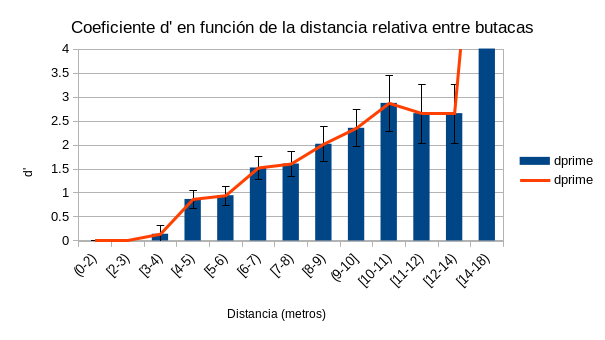
\includegraphics[scale=0.7]{../imagenes/analisisThurstButacasDuda.png}
			    \centering
			    \caption{Coeficientes $d'$ en función de la distancia entre butacas.} 
			    \label{fig:ThurstButacasDuda}
            \end{figure}
            
            \begin{figure}
                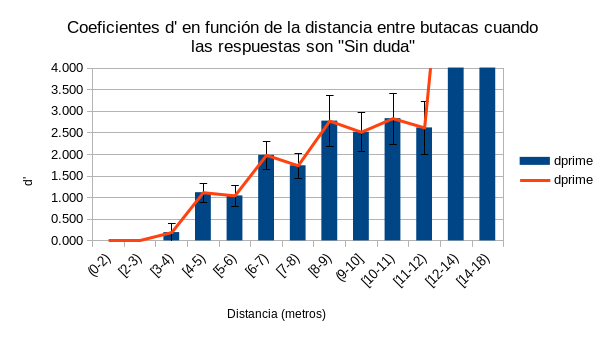
\includegraphics[scale=0.7]{../imagenes/analisisThurstButacasSinDuda.png}
			    \centering
			    \caption{Coeficientes $d'$ en función de la distancia entre butacas cuando las respuestas están marcadas como ``Sin duda''.} 
			    \label{fig:ThurstButacasSinDuda}
            \end{figure}
            
            Al igual que ocurría con los resultados agrupados según la distancia a la fuente, se observa que, a pesar, de que el comportamiento es similar para ambas formas de analizar los datos, la norma UNE-EN ISO 10399 es mucho menos sensible a los pequeños cambios en los resultados; mientras que los modelos thursthonianos ofrecen un rango mayor de datos que fluctúan más facilmente. Esto no es necesariamente peor; depende de lo que se pretenda conseguir con el estudio. Si se pretende determinar a partir de qué distancias las diferencias son significativas, la norma da información más útil en este sentido. Por otro lado, si se pretende estudiar el comportamiento de las diferencias perceptuales en función de la distancia, aquí los modelos thursthonianos tienen una gran ventaja frente a la norma.
    
    \bibliography{biblio}
    \bibliographystyle{babunsrt}
\end{document}